\documentclass{amsart}

\usepackage[margin=1in]{geometry}
\usepackage{amsthm}
\usepackage{amsmath}
\usepackage{amssymb}
\usepackage{bbm}
\usepackage{hyperref}
\usepackage{enumitem}
\usepackage{xcolor}
\usepackage{placeins}
\usepackage{tikz}
\usepackage{graphicx}
\usepackage{algorithm}
\usepackage{algpseudocode}
\usepackage{lineno}

\graphicspath{{figures/}{writeup/figures/}}

\setlength{\parindent}{0pt}
\setlength{\parskip}{0.5em}

\title{Towards stratified sampling for redistricting plans}
\author[ZW, GH, JY, JM, AG]{Zijian Wang, Gregory J. Herschlag, Joon-Hyeok Yim,\\ Jonathan C. Mattingly, and Anna C. Gilbert}
\thanks{%
(ZW) Department of Applied and Computational Mathematics, Yale University, New Haven, CT 06511, USA\\
\indent(GH) Department of Mathematics, Duke University, Durham, NC 27708 USA\\
\indent(JY) Department of Electrical \& Computer Engineering, Yale University, New Haven, CT 06511, USA\\
\indent(JM) Department of Mathematics, Duke University, Durham, NC 27708 USA\\
\indent(AG) Department of Statistics \& Data Science, Yale University, New Haven, CT 06511, USA\\
\indent E-mail addresses: \url{zijian.wang@yale.edu}, \url{gjh@math.duke.edu}, \url{joon-hyeok.yim@yale.edu}, \url{jonm@duke.edu}, \url{anna.gilbert@yale.edu}\\
\indent Date: \today
}


\newtheorem{definition}{Definition}
\newtheorem{remark}{Remark}

\newcommand{\be}{\mathbb{E}}
\newcommand{\bp}{\mathbb{P}}
\newcommand{\br}{\mathbb{R}}
\newcommand{\ind}{\mathbbm{1}}
\newcommand{\rev}[1]{\textcolor{red}{#1}}

%algo name camel case macro
\newcommand{\hccultra}{\textsc{HccUltraFit}}
\newcommand{\beamsearch}{\textsc{BeamSearch}}
\newcommand{\greedysubcover}{\textsc{GreedySubcover}}

\begin{document}
\linenumbers

\begin{abstract}
Rapid algorithmic developments have accelerated the sampling of redistricting ensembles, yet evaluating rare events and sampling complex target measures remains a core challenge due to the high-dimensional and combinatorial nature of the phase space.
To address this and enable variance reduction techniques like stratified sampling, we introduce a scalable computational pipeline to stratify the space of redistricting plans.
We achieve this by clustering districts into representative ``letters'', and then use them to build representative plans (``words'').
A partition of unity over these words corresponds to a soft assignment to a set of strata, allowing us to empirically estimate the flux between strata, as well as stratum weights.
Our work provides a solid foundation for stratified sampling to distributions on redistricting plans.
We demonstrate our computational pipeline using real-world redistricting datasets from Connecticut and North Carolina.
\end{abstract}

\maketitle
\section{Introduction}
Members of the U.S. House of representatives are elected every two years, with a total of $435$ seats apportioned among the states based on population counts from the census~\cite{eckman2019apportionment}.
States that have more than one seat must draw congressional districts and elect one representative per district.
As population distributions shift, district boundary lines are usually redrawn after each census, subject to both federal and state rules.
Since the exact placement of these boundaries can heavily influence election outcomes, the redistricting process is persistently controversial.
Disputes over partisan or racial gerrymandering frequently lead to extensive litigation.
To objectively evaluate whether a redistricting plan has been unfairly manipulated, courts increasingly take into account computational methods~\cite{mattingly2021expert,mattingly2019expert}.

Mathematically, a redistricting plan is a partition of a state's basic geographic or voting units (e.g., precincts) into a fixed number of districts.
These units naturally form a planar graph that encodes geographical contiguity constraints.
A standard way to quantify whether an enacted or proposed redistricting plan is unusual is to compare it against an ensemble of plans that follow similar legal and geographical constraints.
To produce statistically meaningful counterfactuals and hypotheticals, one measures observables of interest~\cite{mattingly2014redistricting,fifield2015new} like voting patterns, demographic distributions, etc., on the ensemble to see whether the enacted plan is typical with respect to the ensemble.
Such ensembles are typically specified via score functions that encode constraints~\cite{mattingly2014redistricting}.
This inspires a large body of work related to drawing ``representative'' redistricting plans ostensibly uniformly at random from all such allowable plans, typically done via MCMC simulations.
Recent algorithmic advances make it feasible to generate large ensembles under increasingly nuanced constraints, for instance, via reversible forest-based merge-split samplers~\cite{autry2020multi,autry2023metropolized} and Cycle Walk~\cite{cyclewalk}.


Despite rapid progress in sampling algorithms, evaluating rare events and exploring complex target measures remains a persistent challenge in the study of redistricting ensembles.
For instance, it is well known that existing samplers exhibit low acceptance rates and slow convergence when the target measure deviates from the tree-count measure~\cite{autry2020multi,cyclewalk}.
To use variance-reduction techniques like stratified sampling, we must first stratify the phase space.
Also known historically in computational chemistry as umbrella sampling~\cite{torrie1977nonphysical}, this approach has become a popular technique for sampling rare events, as well as complex measures~\cite{dinner2020stratification}.
Recent works extend this approach to nonequilibrium sampling via trajectory stratification~\cite{dinner2018trajectory}.
% strata / a set of strata / a stratum
A key prerequisite for stratified sampling is that we need strata that cover the phase space, while maintaining suitable overlaps.
In computational chemistry applications, the underlying phase space is usually an interval, or, more generally a subset of $\mathbb{R}^n$, where there are several canonical ways to construct strata with desired features.
However, it is not immediately clear how to construct such strata over the space of redistricting plans, which is discrete and combinatorial.
Three features make the stratification of redistricting plans particularly challenging: (i) small local boundary moves can produce distinct plans that are, for practical purposes, ``almost the same'', so any useful notion of similarity must capture essential structure while ignoring inconsequential boundary noise; (ii) plans are unordered tuples of districts, so comparing two plans typically requires solving a district-matching problem, which is expensive at scale; and (iii) clustering plans directly can be computationally heavy and may obscure district-level structure, since variation in one district can be largely independent of variation in another.

In this paper, we build a scalable computational pipeline that stratifies redistricting plans. 
We address the aforementioned challenges by first clustering at the district level and then using that structure to build plan-level strata.
This district-level clustering step addresses (i) by grouping together similar districts, and it addresses (iii) by retaining district-level granularity that can be obscured if we directly perform plan-level clustering.
We use a beam-search heuristic to identify, for each plan, a small set of candidate nearest-neighbor words when constructing the strata.
As the first step of the pipeline, we collect districts appearing across the ensemble and cluster them with a hierarchical correlation clustering algorithm \hccultra~\cite{DBLP:journals/corr/abs-2409-01010} under a population-weighted symmetric-difference metric, producing a small ``alphabet'' of representative districts (``letters'').
Each plan is then encoded as an unordered tuple of letters (a ``word'').
Because only a small fraction of all possible words correspond to viable plans, we construct a representative word set near the observed samples from the ensemble via a beam search that expands partial words district-by-district while retaining only the best candidates.
Next, we define a partition of unity (POU) that softly assigns each plan to its nearest words.
In this paper, we provide the framework rather than fixing one specific POU formula, allowing for flexibility when applying this framework to stratified sampling.
In practice, one may need to adjust the weighting according to empirical mixing performance.
Nevertheless, we estimate a stationary distribution over strata and an associated flux matrix with a prescribed POU to demonstrate the plausibility of our method.
We illustrate the pipeline on two real-world examples: Connecticut (small-scale) and North Carolina (large-scale). 
The small-scale Connecticut example provides a better understanding of the words that we construct, since Connecticut only has five districts.
On the other hand, North Carolina has fourteen districts and much more precincts.
We use the North Carolina example to demonstrate the scalability of our pipeline on large-scale datasets.

\medskip
\noindent\textbf{Road map}
%labels compatible with thesis chapter
\begin{itemize}
    \item Section~\ref{sec:chap4 background} provides background on the three ingredients in our pipeline: redistricting ensemble sampling, stratified sampling, and hierarchical clustering.
    \item Section~\ref{sec:chap4 notation_setup} formalizes notation for districts and plans; defines district-level and plan-level distances; introduces letters and words; defines the POU, weights and flux matrix.
    \item Section~\ref{sec:chap4 methodology} details the full pipeline: data generation, hierarchical clustering for building letters, and beam search for candidate words; specifies strategies for choosing alphabet size and word pruning (when overlap is large).
    \item Section~\ref{sec:chap4 numerical_experiments} applies the pipeline to two real-world examples with different sizes (Connecticut and North Carolina).
    \item Section~\ref{sec:chap4 future_directions} discusses next steps, including running full stratified sampling using the strata constructed with the pipeline, and updating the alphabet for new data.
    \item Section~\ref{sec:chap4 conclusion} concludes the paper.
\end{itemize}

\section{Background}\label{sec:chap4 background}

\subsection{Redistricting ensemble sampling}\label{subsec:districting_ensembles}

The idea of using a score-based probability distribution to assess redistricting counterfactual was introduced in $2014$, concurrently by Mattingly and Vaughn~\cite{mattingly2014redistricting} and Fifield et al.~\cite{fifield2015new}.
Tree-based merge-split samplers have quickly emerged as the standard method to draw samples from ensembles of redistricting plans.
In recombination (Recom), one repeatedly merges two adjacent districts, samples a random spanning tree (using Wilson's algorithm via loop-erased random walk), and then cuts an edge to form two new districts that satisfy population balance constraints~\cite{deford2021recombination}.
Since each step produces two entirely new districts from their union, Recom makes relatively global movements comparing to local node flips.
This implies strong empirical mixing properties in practical applications.
It is worth noting that the spanning-tree construction induces an implicit bias toward compact districts~\cite{deford2021recombination}.

A key limitation of vanilla ReCom is that its stationary distribution generally differs from the target measure chosen by the user, e.g., the one proposed in~\cite{mattingly2014redistricting}.
Moreover, using Recom as a Metropolis-Hastings proposal is infeasible because the forward and reverse proposal probabilities are computationally intractable.
The difficulty mainly comes from the fact that a new spanning tree is chosen in each proposal, which drastically increases the number of possible movements.
To address this problem, Metropolized Forest Recom keeps track of spanning forests instead of just partitions, making forward and backward calculations of proposal probabilities viable~\cite{autry2023metropolized}.
Building on this idea, multi-scale merge-split methods further extend the state space to a forest of tree hierarchies, which has improved scaling properties and is useful for handling county constraints~\cite{autry2020multi}.

In contrast to merge-split proposals that completely resamples a pair of districts, Cycle Walk operates directly on spanning forests using cycle-based local updates: it adds an edge to create a cycle and then removes another edge at random to break the cycle~\cite{cyclewalk}.
This produces relatively local moves comparing to the methods discussed earlier.
The resulting chain can be Metropolized to target a user-specified distribution.
In numerical studies, it shows good convergence performance on examples that are challenging for existing Recom-type algorithms.
In this paper, we use Cycle Walk to generate the redistricting plans as input to our computational pipeline.



\subsection{Stratified Sampling}\label{subsec:umbrella_mbar}
Stratified sampling is a variant of importance sampling that was developed in computational chemistry to overcome the inefficiencies of vanilla Monte Carlo methods.
Originally introduced in the work by Torrie and Valleau to compute free-energy differences under the name umbrella sampling~\cite{torrie1977nonphysical}, the method and its many extensions~\cite{kumar1992weighted,shirts2008statistically} are increasingly formalized in modern statistical literature as stratified samplking or stratified MCMC methods~\cite{dinner2018trajectory}.
One core challenge in these type of problems is that the chain rarely cross large free-energy barriers, making it hard to sample complex measures and rare-events~\cite{kastner2011umbrella,kumar1992weighted}.
This challenge closely mirrors the algorithmic bottlenecks when sampling redistricting plans.
It is known that Recom-type algorithms exhibit prohibitively low accepantace rate when the targeting measure deviates from the tree-count measure~\cite{autry2020multi}.
While newer approaches like Cycle Walk~\cite{cyclewalk} shows empirical improvement, convergence on general measures is still relatively slow.

Stratified sampling addresses this by splitting $\pi$ into easier-to-sample distributions $\{\pi_s\}_{s\in\mathcal{S}}$.
To obtain these distributions, we tilt $\pi$ by nonnegative functions $\{\rho_s\}_{s\in\mathcal{S}}$:
\begin{align}
    \pi_s(x):=\frac{1}{z_s}\rho_s(x)\pi(x),
\end{align}
where $z_s$ is the partition function that normalizes $\pi_s$ into a probability distribution.
The functions $\rho_s$ are designed to cover the phase space, including the low-probability regions, while maintaining overlap to allow for communication between different $\pi_s$.
The main challenge for this type of methods is to find the normalization terms $z_s$.
Let $z$ be the vector formed by concatenating $z_s$.
The following fact about $z$ can be verified via straightforward matrix multiplication:
\begin{align}\label{eqn: umbrella fixed point}
    zG(z)=z,\quad\quad G_{s,s'}(z):=\mathbb{E}_{\pi_s}\left[\frac{\rho_{s'}/z_{s}}{\sum_{t}\rho_{t}/z_{t}}\right].
\end{align}
The above implies that $z$ is a left eigenvector of $G(z)$ with eigenvalue one.
This provides a fixed-point iteration approach to solve $z$ by alternating between updating $G$ and evaluating its left eigenvector $z$, which is essentially the basis of the eigenvector method for umbrella sampling (EMUS)~\cite{dinner2020stratification,matthews2018umbrella}.

Alternatively, one can construct stratified sampling from a soft assignment viewpoint, which forms a more general mathematical framework that easily extends to nonequilibrium sampling~\cite{dinner2018trajectory}.
Suppose we have a set of strata $\mathcal{S}$ equipped with a partition of unity (POU) on the phase space $\{\phi_s\}_{s\in \mathcal{S}}$, which can be viewed as a type of ``soft assignment'' to the strata.
A common way to obtain a set of POU is to start with functions $\psi_s(x)$ and normalize them:
    \begin{align}
        \phi_s(x):=\frac{\psi_s(x)}{\sum_{s\in\mathcal{S}}\psi_s(x)},\quad\quad x\in X.
    \end{align}
This computation is tractable as long as each $x$ is only in the support of $\psi_s$ for a small number of $s$.
Using the POU, we can define stratum weights and a flux matrix via
    \begin{align}
        z_s:=\mathbb{E}_\pi[\phi_s],\quad\quad F_{s,s'}:=\mathbb{E}_{\pi_s}[\phi_{s'}].
    \end{align}
Note that expanding $F_{s,s'}$ using $\phi_s$ gives us an equation that is similar to \eqref{eqn: umbrella fixed point}.
However, the flux matrix $F$ constructed in this way is row-stochastic, whereas $G$ is not in general.
One advantage of using this POU approach is that we can view it as the transition kernel of a Markov chain on the set of strata.



\subsection{Hierarchical clustering}\label{subsec:hierarchical_clustering}
Note that the space of redistricting plans is complex, hence it is generally hard to define meaningful strata.
To address this, we analyze the space of individual districts using hierarchical clustering.
Let $\mathcal{X}=\{x_1,x_2,\dots x_N\}$ be a dataset of size $N$, and $D\in\mathbb{R}^{N\times N}$ be the pairwise distances.
A hierarchical clustering algorithm maps $D$ to an ultrametric distance matrix $D_T$.
The resulting output of a hierarchical clustering algorithm can be viewed in several mathematically equivalent ways: a nested sequence of partitions on $\mathcal{X}$, a binary tree with $N$ leaves (a dendrogram), or an ultrametric topology on $\mathcal{X}$~\cite{murtagh2012algorithms}. 

The nodes of a dendrogram are subsets of $\mathcal{X}$, which can also be viewed as clusters of data points.
In a dendrogram, singleton leaves $\{x_i\}$ gradually merge until they form the root $\mathcal{X}$.
By construction, any two nodes within a dendrogram are either completely disjoint, or one is entirely contained within the other.
The vertical axis of a dendrogram represents the ultrametric distance, a metric that satisfies the strong triangle inequality:
    \begin{align}
        d(x_i,x_j)\leq\max(d(x_i,x_k),d(x_j,x_k)),\quad\quad x_i,x_j,x_k\in\mathcal{X}.
    \end{align}
This condition implies that the distance between any two leaves is simply the height of their lowest common ancestor in the dendrogram.
To extract a clustering of size $K$, one simply ``cuts'' the dendrogram at a specific threshold.
In other words, we discard the edges above the threshold, allowing the sub-trees below the threshold to form a size-$K$ partition of $\mathcal{X}$.
See Figure \ref{fig:dendro_example} for an example of a dendrogram, as well as the cutting procedure.
\begin{figure}[!htbp]
    \centering
    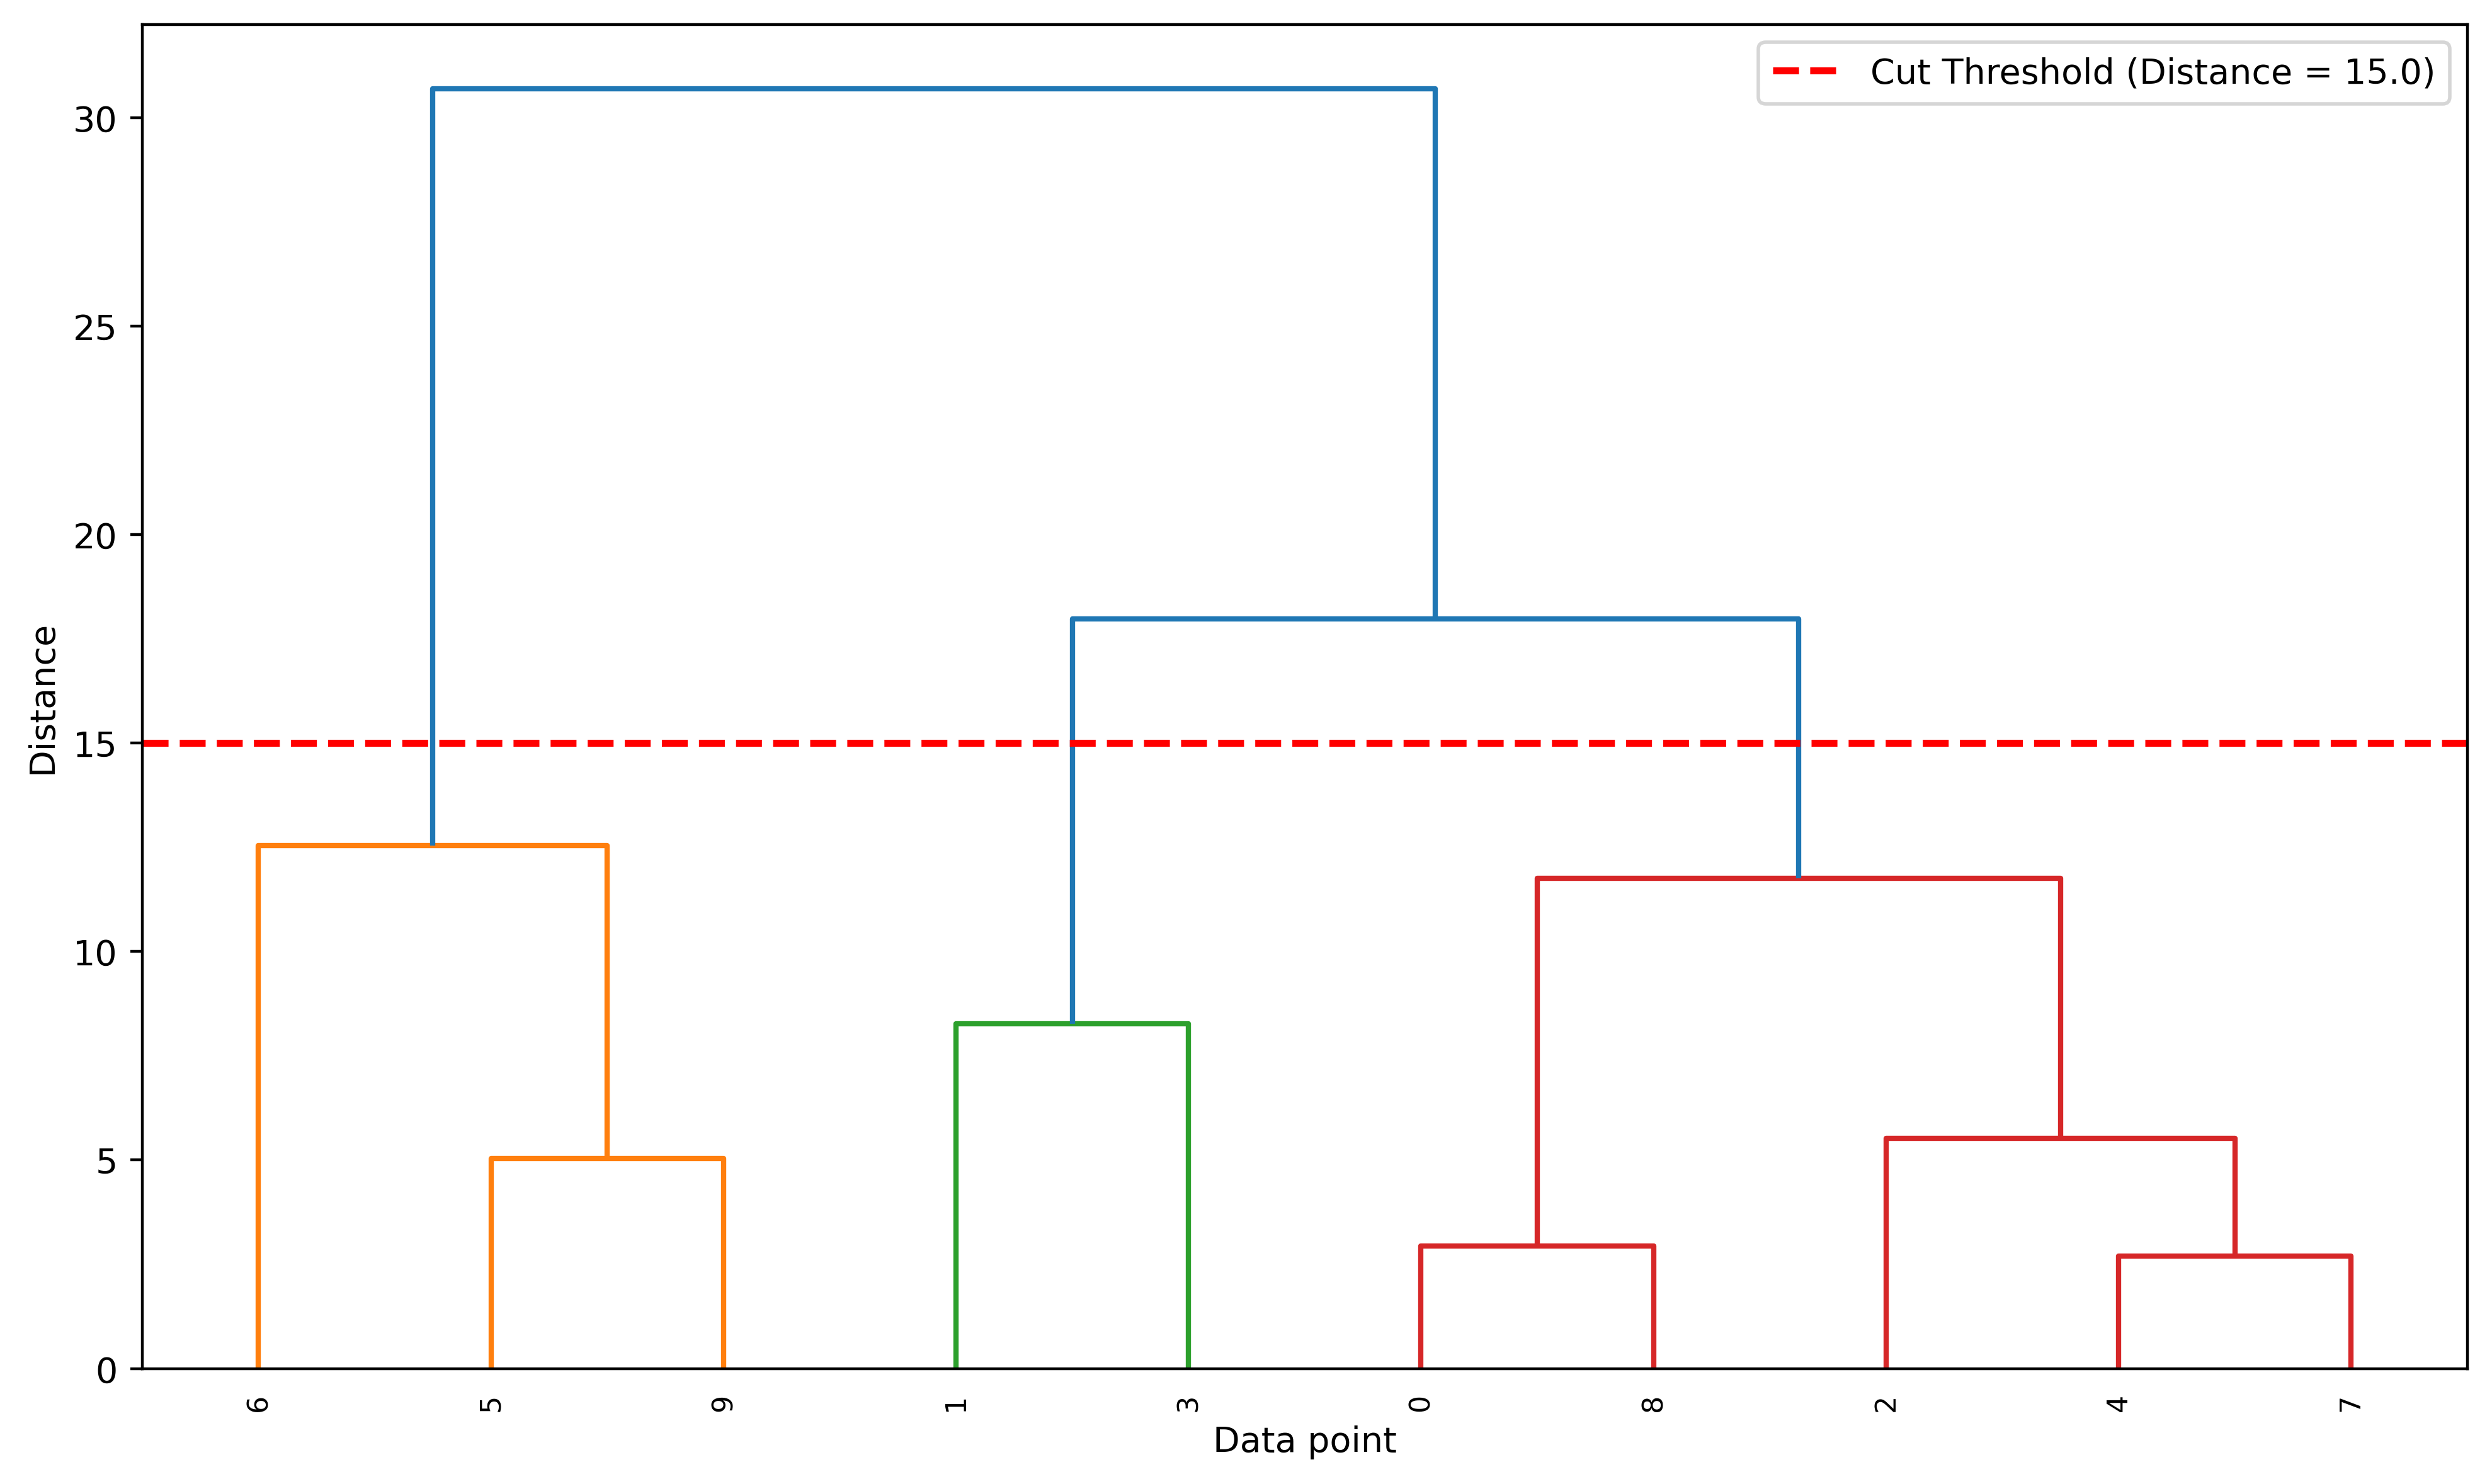
\includegraphics[width=0.8\linewidth]{figures/dendro_example.png}
    \caption{Example dendrogram: $x$-axis shows the indices of data points ($10$ in total), $y$- axis shows the ultrametric distance. The red dashed line indicates a cut at distance $15$, producing three clusters (colored in orange, green and red).}
    \label{fig:dendro_example}
\end{figure}

Classical strategies for building the dendrogram typically involve greedy and irreversible steps that merge the closest pair of clusters at each step based on a heuristic linkage criterion (e.g., single, complete or average linkage)~\cite{sibson1973slink,defays1977efficient,sokal1958statistical}.
While these linkage criteria are easy to implement, they typically do not capture the underlying geometry of the dataset due to their heuristic nature, i.e., ultrametric induced by the dendrogram may be far from the original distances.
In contrast, \hccultra~\cite{DBLP:journals/corr/abs-2409-01010} addresses this problem by proposing a hierarchical correlation clustering algorithm. 
This method fits an ultrametric to $\mathcal{X}$ with a theoretical guarantee on the number of disagreement pairs across every partition level. 
Such consistency across the hierarchy is not observed in common linkage based methods. 
Although the primary goal of \hccultra in~\cite{DBLP:journals/corr/abs-2409-01010} is to manage ultrametric distances, our computational pipeline specifically utilizes their implementation to generate district clusters. Note that we only use the dendrogram output of \hccultra, but the original paper~\cite{DBLP:journals/corr/abs-2409-01010} has a much wider scope.

\section{Problem setup and notation}\label{sec:chap4 notation_setup}

Let $V:=[P]$ be the set of basic geographic/voting units in a U.S. state and let $w_1,w_2,\dots,w_P$ be the population in each unit.
The map of the U.S. state induces a graph $G=(V,E)$, where two vertices are connected if they are geographically adjacent.
A congressional plan is a partition of the set of precincts $V$ into $I$ districts, where $I$ is determined by the number of U.S. House seats the state has after apportionment~\cite{eckman2019apportionment}.
At a high level, a plan is admissible if it satisfies a number of constraints.
For instance, it needs to be balanced (up to a certain population deviation threshold) and satisfy contiguity (i.e. geographically connected).

It is convenient to view a district $v$ as a vector that lives in $\mathcal{V}\subset\{0,1\}^P$, where
\begin{align}
v_p =
    \begin{cases}
    1, & \text{if } p\text{ is in the district},\\
    0, & \text{otherwise.}
    \end{cases}
\end{align}
Let $\mathcal{W}:=\mathcal{V}^I/S_I$ be the space of unordered $I$-tuples from $\mathcal{V}$ and let $\mathcal{X}\subset\mathcal{W}$ be the subset of admissible plans.
A natural way to define a distance $\mathcal{V}\times\mathcal{V}\to\mathbb{R}$ between two districts $v$ and $v'$ is via a capped population-weighted $\ell^1$:
\begin{align}\label{eq:dist_district}
    d(v,v') := \min\Big(d_{\max}, \sum_{p=1}^{P}|v_p -v'_p|\,w_p\Big).
\end{align}
We include a distance upper bound $d_{\max}>0$ to reduce the noise when two districts are disjoint.
A common choice for the cap is 
\begin{align}
d_{\max}=\frac{2}{I}\sum_{p=1}^{P} w_p.
\end{align}
We can extend the distance on $\mathcal{V}$ to a distance function on plans $\mathcal{W}$ by taking the minimum over all matchings:
\begin{align}\label{eq:dist_plan}
    D(w,w')
    := \min_{\pi\in S_I}\sum_{i=1}^I d\big(w_i,w'_{\pi(i)}\big).
\end{align}
One of the central themes in this paper is to systematically identify plans that are similar.
Instead of working with plans directly, we start by identifying similar districts and use that information to reduce the complexity of the plan-level problem. 
In the three redistricting plans shown in Figure \ref{fig:letter_district_example}, we see that the districts in the southwest corner of Connecticut (which includes Fairfield County) are similar to each other, while the rest of the state has drastically different districting patterns.
\begin{figure}[!htbp]
    \centering
    
\includegraphics[width=1.0\linewidth]{figures/letter_district_example.png}
    \caption{Letter/cluster example based on redistricting samples from Connecticut. From left to right, we have: 1. Fraction of districts containing each precinct; 2. The letter as the centroid of the cluster; 3-5. Plans that contain districts similar to the letter (highlighted in red).}
    \label{fig:letter_district_example}
\end{figure}
\FloatBarrier
To identify districts similar to those in Figure \ref{fig:letter_district_example}, we form $K$ clusters on the district space and reduce the complexity of plans by identifying each district by its centroid.
Given a cluster of districts $\tilde{\mathcal{V}}\subset \mathcal{V}$, we define the centroid $\tilde v$ to be the point in $\{0,1\}^P$ that minimizes the average uncapped weighted $\ell^1$ distance to all points in $\tilde{\mathcal{V}}$.
Under this centroid objective, letters are naturally zero-one valued even if we relax the optimization over $[0,1]^P$.
However, letters are not guaranteed to be an existing district.
An alternative approach is to restrict the distance optimization problem to $\mathcal{V}$.
In this paper, we call these centroids letters.
Using $K$ clusters, we obtain an alphabet of size $K$ and can use these letters to form words, which are unordered tuples of letters of fixed size $I$.
Note that letters are objects in $\{0,1\}^P$ and words are objects in $\mathcal{W}$.

Even after the reduction in district space, we still have an exponentially large word space.
Observe that the space of words relevant to actual plans in the ensemble is much smaller.
For instance, we are not interested in words with repeated letters, assuming that the underlying alphabet forms a good representation of the districts.
Based on this observation, we further reduce the space of words by keeping only the $L$ nearest candidate words for each observed plan $x\in\mathcal{X}$ under $D$ (computed via a beam search with width $L$ in Section~\ref{sec:chap4 methodology}).
We then work with the union of these candidate sets, which yields a manageable representative word set that is convenient for downstream tasks, e.g. stratified sampling.

Let $\mathcal{S}\subset\mathcal{W}$ be a representative set of words, which forms a set of strata over the space of plans.
We construct a soft assignment of plans to strata using a partition of unity (POU) $\{\phi_s\}_{s\in \mathcal{S}}$ over plans $x\in\mathcal{X}$:
\begin{align}\label{eq:pou}
    \sum_{s\in \mathcal{S}}\phi_s(x)=1,\qquad
    \phi_s(x):=\frac{\psi(x;s)}{\sum_{s'\in \mathcal{S}}\psi(x;s')}.
\end{align}
For each plan $x$, let $\mathcal{N}_{\mathcal{S}}(x)\subseteq\mathcal{S}$ denote the retained word neighborhood for that plan, typically the words in $\mathcal{S}$ that appear among its $L$ nearest beam-search candidates.
Note that $\mathcal{N}_{\mathcal{S}}(x)$ is often smaller than the beam-width due to pruning.
We define $\psi$ by
\begin{align}\label{eq:psi_relative}
    \psi(x;s)=
    \begin{cases}
        \exp\!\big(-T\kappa(D(x,s))), & s\in\mathcal{N}_{\mathcal{S}}(x),\\
        0, & \text{otherwise,}
    \end{cases}
\end{align}
where $T\geq 0$ is a temperature parameter controlling sensitivity to distances and $\kappa$ is an $\mathbb{R}\to\mathbb{R}$ function that maps distances (in units of population) into appropriate ranges.
When $T=0$, the function $\psi$ assigns equal unnormalized weights to the retained words of a given plan $x$.
% internal comment: T=0 is what we use for proof of principles. This avoids complication from choice of kappa.
Let $\pi$ be the target distribution on plans.
We define the stratum weights by
\[
    z_s := \mathbb{E}_{\pi}[\phi_s],
\]
and the flux matrix between strata by
\begin{align}\label{eq:flux}
    F_{s,s'} := \mathbb{E}_{\pi_s}[\phi_{s'}]
    = \frac{1}{z_s}\mathbb{E}_{\pi}[\phi_s\phi_{s'}],
    \qquad \text{where } \frac{d\pi_s}{d\pi}=\frac{1}{z_s}\phi_s.
\end{align}
By construction, $F$ is row-stochastic and $z$ is stationary for $F$ (i.e., a left eigenvector with eigenvalue $1$).
Observe that this setup is consistent with the standard US framework, see, e.g. \eqref{eqn: umbrella fixed point}.


We conclude this section with a table of notation.
\begin{table}[!htbp]
    \centering
    \small
\renewcommand{\arraystretch}{1.1}
\begin{tabular}{ll}
    \hline
    Symbol & Meaning \\
    \hline
    $G=(V,E)$ & Precinct adjacency graph \\
    $P$ & Number of precincts ($|V|$) \\
    $V$ & Precinct vertex set ($V=[P]$) \\
    $E$ & Adjacency edge set \\
    $\mathcal{V}$ & District indicator space \\
    $\mathcal{W}$ & Space of unordered $I$-tuples of $\mathcal{V}$ \\
    $\mathcal{X}$ & Admissible plan space \\
    $x$ & A plan in $\mathcal{X}$ \\
    $w_p$ & Population weight of precinct $p$ \\
    $I$ & Number of districts in a plan \\
    $d_{\max}$ & Cap used in $d$ \\
    $d$ & District-level distance \eqref{eq:dist_district} \\
    $D$ & Plan-level distance \eqref{eq:dist_plan} \\
    $K$ & Number of letters (district clusters) \\
    $l$ & A letter (cluster centroid) \\
    $L$ & Word degree (number of candidates kept) \\
    $\mathcal{S}$ & Representative word set / strata \\
    $s$ & A stratum (word) in $\mathcal{S}$ \\
    $w_i(x)$ & $i$-th nearest word to plan $x$ \\
    $\psi(x;s)$ & Unnormalized kernel \eqref{eq:psi_relative} \\
    $\phi_s(x)$ & POU weight \eqref{eq:pou} \\
    $T$ & Temperature parameter in \eqref{eq:psi_relative} \\
    $\pi$ & Target distribution on plans \\
    $\pi_s$ & Stratum distribution \eqref{eq:flux} \\
    $z_s$ & Stratum weight $\be_{\pi}[\phi_s]$ \\
    $F_{s,s'}$ & Flux matrix \eqref{eq:flux} \\
    \hline
\end{tabular}
\caption{Summary of basic notations.}
\label{tab:notation}
\end{table}


\section{Methodology}\label{sec:chap4 methodology}

\subsection{Data generation}
We study ensembles of redistricting plans $x$ distributed according to a measure of interest:
    \begin{align}
        \pi(x)\propto e^{-J(x)},
    \end{align}
where $J$ is a score function that reflects the hard and soft constraints for a desirable redistricting plan, e.g., population deviation, connectedness, etc.
To efficiently obtain plan samples from $\pi$, we use the Metropolized Cycle Walk~\cite{cyclewalk}.
Each step modifies a spanning forest (on $G$) by adding an edge $e$ and removing a random edge on the cycle created by $e$.
We then accept or reject the resulting forest using a standard Metropolis-Hastings acceptance rule that satisfies detailed balance.
After burn-in, we collect $M$ observations $\mathcal{X}_{obs}:=\{x^{(m)}\}_{m=1}^M$ from the chain output every $100$ steps.

Recall that each plan $x^{(m)}$ is an unordered tuple of $I$ districts in $\mathcal{V}$. 
Pooling districts across the $M$ plans yields a set of $N$ districts
\begin{align}
    \mathcal{D} := \{v_1,\dots,v_N\}\subset \mathcal{V},
\end{align}
where $N\leq MI$ because plans may contain exactly same districts.
We compute the pairwise district-to-district distances according to \eqref{eq:dist_district} and store them in coordinate (COO) format, which is convenient for the clustering algorithms that we use.
This approach saves memory because we only store the distances below $d_{max}$, especially when $I$ is large.

\subsection{Building letters}
To find representative districts (``letters''), we cluster the pooled district set $\mathcal{D}$ with \hccultra~\cite{DBLP:journals/corr/abs-2409-01010}, which is a hierarchical correlation clustering algorithm that comes with nice theoretical guarantees.
To scale the algorithm to large graphs, we optimize memory usage by tracking only the active roots during merging, which avoids storing a dense $2N\times 2N$ matrix as in a naive implementation.
The most time-consuming step is sorting the edges by distance.
We therefore bucket-sort the COO distances and parallelize across bins, where bin boundaries are estimated from a small pilot sample.
This produces a single dendrogram, which we can cut to obtain clustering for any desired $K$.

To choose $K$, we use the elbow method on a dispersion objective $\mathcal{L}(K)$.
Let $\mathcal{D}_1,\mathcal{D}_2,\dots,\mathcal{D}_K$ be the clusters, i.e., a partition of $\mathcal{D}$.
For each cluster, we define its letter (centroid) $l_k\in\{0,1\}^P$ as the point that minimizes the sum of distances to members of $\mathcal{D}_k$:
\begin{align}\label{eq:centroid definition}
    l_k &:= \arg\min_{l\in\{0,1\}^P}\sum_{v\in\mathcal{D}_k}d(l,v),\\
\end{align}
Under weighted $l^1$ distance \eqref{eq:dist_district}, this reduces to a precinct-wise median:
\begin{align}
    (l_k)_p &=
    \begin{cases}
        1, & \sum_{v\in\mathcal{D}_k} v_p \ge \frac{|\mathcal{D}_k|}{2},\\
        0, & \text{otherwise,}
    \end{cases}
    \qquad p=1,\dots,P.
\end{align}
Given the letters $l_1,\dots,l_K$, we score the clustering via the within-cluster dispersion
\begin{align}\label{eq:dispersion_obj}
    \mathcal{L}(K) &:= \sum_{k=1}^K \sum_{v\in\mathcal{D}_k} d(v,l_k),
\end{align}
an $\ell^1$ analogue of within-cluster sum of squares (WCSS), which is a common metric for choosing the number of clusters.
Empirically, we find that $\mathcal{L}(K)$ is strongly correlated with standard alternatives such as the Silhouette score, the Calinski--Harabasz index, and BCSS, as well as information-theoretic objectives like BIC and AIC.

\subsection{From letters to words}\label{subsec:letters_to_words}
After clustering districts into an alphabet $\{l_1,\dots,l_K\}$, we construct the set of words by taking the union of unordered $I$-tuples of letters around each plan $x\in\mathcal{X}$.
These candidate words serve two roles: they provide a compressed description of the plans, and they define the local support of the kernel $\psi$ in \eqref{eq:psi_relative} used for the partition of unity.
Observe that evaluating the plan-level distance \eqref{eq:dist_plan} between two arbitrary elements of $\mathcal{W}$ is computationally intractable, since it involves looping over all permutations of size $I$.
However, we can exactly enumerate $L$ closest neighbors for a point in $\mathcal{W}$ in $\mathcal{O}(IK\log L+K\log K)$ via beam search.

Let $v_1(x),\dots,v_I(x)$ be the districts of $x$.
For each district, we precompute a sorted list of letter candidates
\begin{align}\label{eq:district_to_letter_candidates}
    C_i(x) &:= \big(d_{v_i(x),l_k},l_k\big)_{k=1}^K,\qquad i=1,\dots,I,
\end{align}
where the pairs are sorted by increasing $d_{v_i(x),l_k}$.
During beam search, we incrementally build partial sub-words by adding one letter at a time, and keep only the $L$ best candidates at each step.
See Algorithm~\ref{alg:beam_search} for more details.
\begin{algorithm}[!htbp]
\caption{Beam search for nearest words with width $L$}
\label{alg:beam_search}
\begin{algorithmic}[1]
\Require For each district $i\in[I]$, a list $C_i=\{(d_{i,k}, \ell_{i,k})\}_{k=1}^K$ of candidate letters sorted by $d_{i,k}$
\State $B \gets [(0, [])]$ \Comment{beam of (distance, partial word)}
\For{$i=1$ \textbf{to} $I$}
    \State $H \gets$ empty max-heap keyed by negative distance \Comment{keeps track of $L$ minimum distances}
    \ForAll{$(D,s)\in B$}
        \ForAll{$(d,\ell)\in C_i$}
            \If{$\ell \in s$}
                \State \textbf{continue} \Comment{avoid repeated letters}
            \EndIf
            \State $D' \gets D + d$
            \State $s' \gets \mathrm{append}(s,\ell)$
            \State \Call{HeapPush}{$H,(D',s')$}
            \If{$\Call{HeapSize}{H} > L$}
                \State \Call{HeapPopMax}{H} \Comment{discard the current worst (largest-distance) candidate}
            \EndIf
        \EndFor
    \EndFor
    \State $B \gets$ elements of $H$ sorted by increasing distance
\EndFor
\State \Return $B$
\end{algorithmic}
\end{algorithm}

\begin{figure}[!htbp]
    \centering
    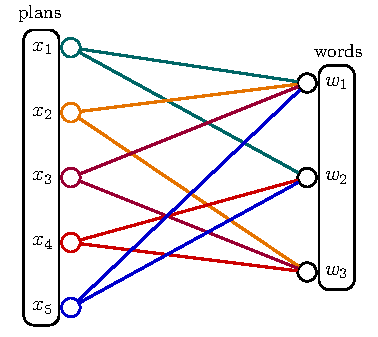
\includegraphics[width=0.55\linewidth]{figures/overlap/bipartite.pdf}
    \caption{Connectivity of a beam search with width $2$. Edges are colored by plans. Each observed plan on the left connects to the two closest words. In this example, we obtain three words in total.}
    \label{fig:overlap/bipartite}
\end{figure}
\FloatBarrier
For each observed plan $x$, we keep the $L$ best candidates as $w_1(x),\dots,w_L(x)$ and take the union of these sets across the ensemble to form the representitative word set $\mathcal{S}$ used for stratification.
It maybe helpful to treat plans and words as vertices and think of the beam search process as building the connections in a bipartite graph, as shown in Figure \ref{fig:overlap/bipartite}.

\subsection{Towards stratification}
The representative word set $\mathcal{S}$ and the plan-level distances $D$ allow us to construct a stratification of the target distribution $\pi$ on plans.
We start with a partition of unity (POU) $\{\phi_s\}_{s\in\mathcal{S}}$ and define the corresponding stratum distributions $\{\pi_s\}_{s\in\mathcal{S}}$ via tilting.
Each $\phi_s(x)$ can be interpreted as a soft-assignment of plan $x$ to stratum $s$, with flow between strata encoded by the flux matrix $F$ in \eqref{eq:flux}.

One key requirement for US to work is coverage, meaning that every plan should have at least one nearby word so that the POU is well-supported.
In our construction this is ensured by beam search, which yields $L$ candidate words $w_1(x),\dots,w_L(x)$ for each plan $x$ and restricts $\psi(x;s)$ in \eqref{eq:psi_relative} to this neighborhood.
Another important requirement of US is that strata have appropriate overlaps.
Some overlap is necessary for communication between strata, but excessively large overlap can lead to slow convergence (as well as numerical instability) of EMUS-style fixed-point iterations.
In practice, the temperature $T$ and the choice of $\kappa$ in \eqref{eq:psi_relative} are the primary control knobs that we can tune to reach desired coverage and overlap.
By construction, the induced coarse dynamics on $\mathcal{S}$ has stationary distribution $z$:
\begin{align}
    \pi(x) &= \sum_{s\in\mathcal{S}} z_s\,\pi_s(x),\qquad
    z^\top F = z^\top,
\end{align}
which we use as a diagnostic to see whether the strata design is fit for stratified sampling.

Actually running stratified sampling requires additional sampling work (e.g., parallel chains targeting $\{\pi_s\}$), whereas here we focus on setting up a reasonable stratification of plan space and the associated overlap statistics.
When overlap is very large and $\mathcal{S}$ becomes highly redundant, we may prune the strata by solving a set-cover problem induced by the plan--word bipartite graph.
Concretely, each word covers a subset of the observed plans, so the words define a family of subsets of the plan space.
The basic greedy subcover routine takes a boolean adjacency matrix $A\in\{0,1\}^{M\times|\mathcal{S}|}$ and repeatedly adds the word that covers the largest number of currently uncovered plans.
Selecting a minimum-size sub-collection $\mathcal{S}_0\subseteq\mathcal{S}$ can be written as
\begin{align}
    \min_{\mathcal{S}_0\subseteq\mathcal{S}} \quad & |\mathcal{S}_0|,\\
    \text{s.t.}\quad & \sum_{s\in\mathcal{S}_0} A_{m,s} \ge 1,\qquad m=1,\dots,M.
\end{align}
The problem of deciding whether there is a subcover smaller than some fixed size is NP-complete in general, so we use the greedy approximation in Algorithm~\ref{alg:greedy_subcover}.
\begin{algorithm}[!htbp]
\caption{Greedy subcover}
\label{alg:greedy_subcover}
\begin{algorithmic}[1]
\Require Adjacency matrix $A\in\{0,1\}^{M\times|\mathcal{S}|}$
\State $U \gets \{1,\dots,M\}$ \Comment{uncovered plan indices}
\State $R \gets \mathcal{S}$ \Comment{remaining candidate words}
\State $\mathcal{S}_0 \gets \emptyset$
\While{$U\neq\emptyset$ and $R\neq\emptyset$}
    \ForAll{$s\in R$}
        \State $g(s) \gets \sum_{m\in U} A_{m,s}$ \Comment{number of newly covered plans}
    \EndFor
    \If{$\max_{s\in R} g(s)=0$}
        \State \textbf{break}
    \EndIf
    \State pick any $s^\star \in\arg\max_{s\in R} g(s)$
    \State $\mathcal{S}_0 \gets \mathcal{S}_0 \cup \{s^\star\}$
    \State $U \gets \{m\in U: A_{m,s^\star}=0\}$ \Comment{remove newly covered plans}
    \State $R \gets R\setminus\{s^\star\}$
\EndWhile
\State \Return $(\mathcal{S}_0,U)$ \Comment{$U=\emptyset$ when $A$ is fully covered}
\end{algorithmic}
\end{algorithm}


In our setting, the adjacency matrix is obtained by thresholding plan--word distances, so the choice of radius matters.
A large radius improves coverage but may connect plans to distant words, while a small radius gives tighter strata but may leave some observed plans uncovered.
Let $D$ be the plan-to-word distance matrix.
We set the larger threshold to the worst nearest-word distance over all plans,
\begin{align}
    \tau:=\max_m\min_{s\in\mathcal{S}}D_{m,s},
\end{align}
so every observed plan is covered at radius $\tau$.
We parameterize the smaller threshold by the ratio $\eta\in(0,1)$ and set $\tau':=\eta\tau$.
Thus, $\eta$ is the only parameter that needs to be chosen.
The two thresholds define adjacency matrices
\begin{align}
    A_{\tau'}:= \ind\{D\leq \tau'\},\quad\quad A_\tau:= \ind\{D\leq \tau\},
\end{align}
where the indicator function is applied element-wise.
The first greedy subcover at radius $\tau'$ gives $\mathcal{S}_{\tau'}$.
If any plans remain uncovered, the second greedy subcover at radius $\tau$ is restricted to those plans and to words not selected in the first stage, and gives $\mathcal{S}_\tau$.
We define the pruned set as
\begin{align}
    \mathcal{S}_\eta:=\mathcal{S}_{\tau'}\cup\mathcal{S}_\tau.
\end{align}
Algorithm~\ref{alg:eta_greedy_subcover} summarizes this two-stage procedure.
\begin{algorithm}[!htbp]
\caption{Two-stage greedy subcover with parameter $\eta$}
\label{alg:eta_greedy_subcover}
\begin{algorithmic}[1]
\Require Distance matrix $D\in\mathbb{R}^{M\times|\mathcal{S}|}$; total population $W$; threshold parameter $\eta>0$
\State $\tau \gets\max_m \min_{s\in\mathcal{S}}D_{m,s}$
\State $\tau_\eta \gets \eta W$
\State $A_{\tau_\eta}\gets\ind\{D\leq\tau_\eta\}$
\State $A_\tau\gets\ind\{D\leq\tau\}$
\State $(\mathcal{S}_{\tau_\eta},U_{\tau_\eta}) \gets \Call{GreedySubcover}{A_{\tau_\eta}}$
\State $A_\tau^{\mathrm{rem}}\gets A_\tau$ restricted to rows $U_{\tau_\eta}$ and columns $\mathcal{S}\setminus\mathcal{S}_{\tau_\eta}$
\State $(\mathcal{S}_\tau,U_\tau) \gets \Call{GreedySubcover}{A_\tau^{\mathrm{rem}}}$
\State $\mathcal{S}_\eta \gets \mathcal{S}_{\tau_\eta}\cup\mathcal{S}_\tau$
\State \Return $\mathcal{S}_\eta$
\end{algorithmic}
\end{algorithm}


We end this section by summarizing the methods we use in our analysis pipeline as a flowchart in Figure \ref{fig:overlap/pipeline_flowchart}.
\begin{figure}[!htbp]
    \centering
    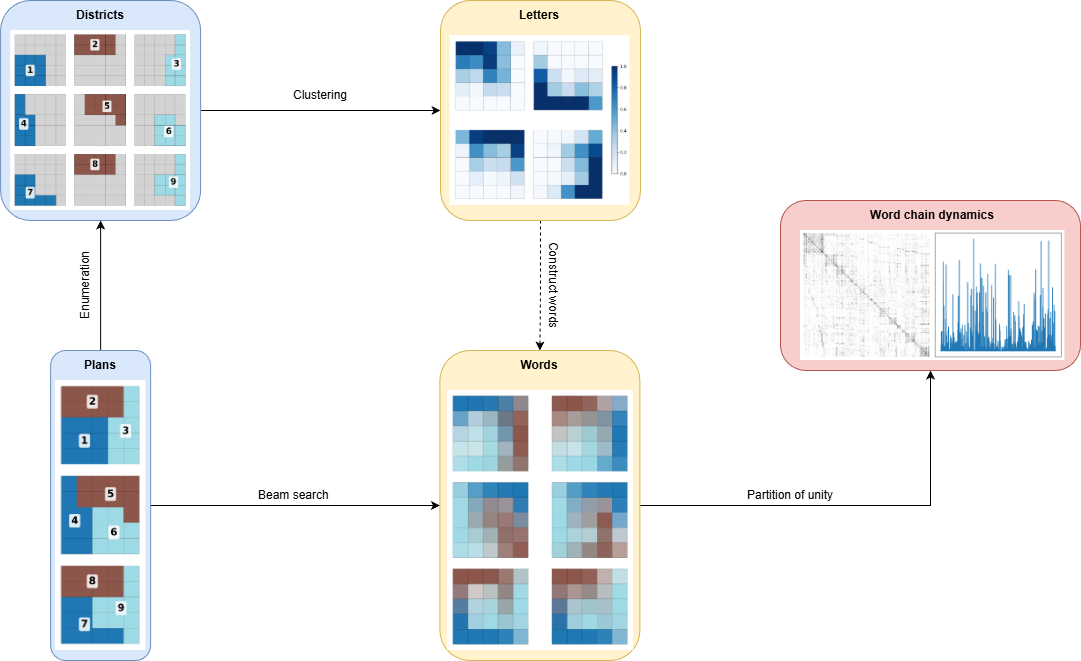
\includegraphics[width=0.92\linewidth]{figures/pipeline_flowchart.png}
    \caption{Overview of the pipeline: districts pooled from an ensemble are clustered into representative district types (letters), each plan is encoded as a unordered tuple of letters (a word), and a beam search enumerates a small neighborhood of candidate words around each plan. A partition of unity over the representative word set then yields stratum weights and a flux matrix summarizing coarse dynamics on words.}
    \label{fig:overlap/pipeline_flowchart}
\end{figure}
\FloatBarrier

\section{Numerical Experiments}\label{sec:chap4 numerical_experiments}
In this section, we demonstrate our pipeline using a small-scale real-world example on Connecticut with five districts $|V|=462,|I|=5$.
The data we use is obtained from the VEST project~\cite{mcdonald2008united} via~\cite{redistrictingdatahub}.
\subsection{Exploratory analysis}\label{sec:connecticut}
We apply the pipeline to redistricting plans of Connecticut, where $|V|=462$ precincts are partitioned into $I=5$ congressional districts.
See Figure \ref{fig:ct_enacted_pop} for the enacted plan in $2022$ and population distribution.
\begin{figure}[!htbp]
    \centering
    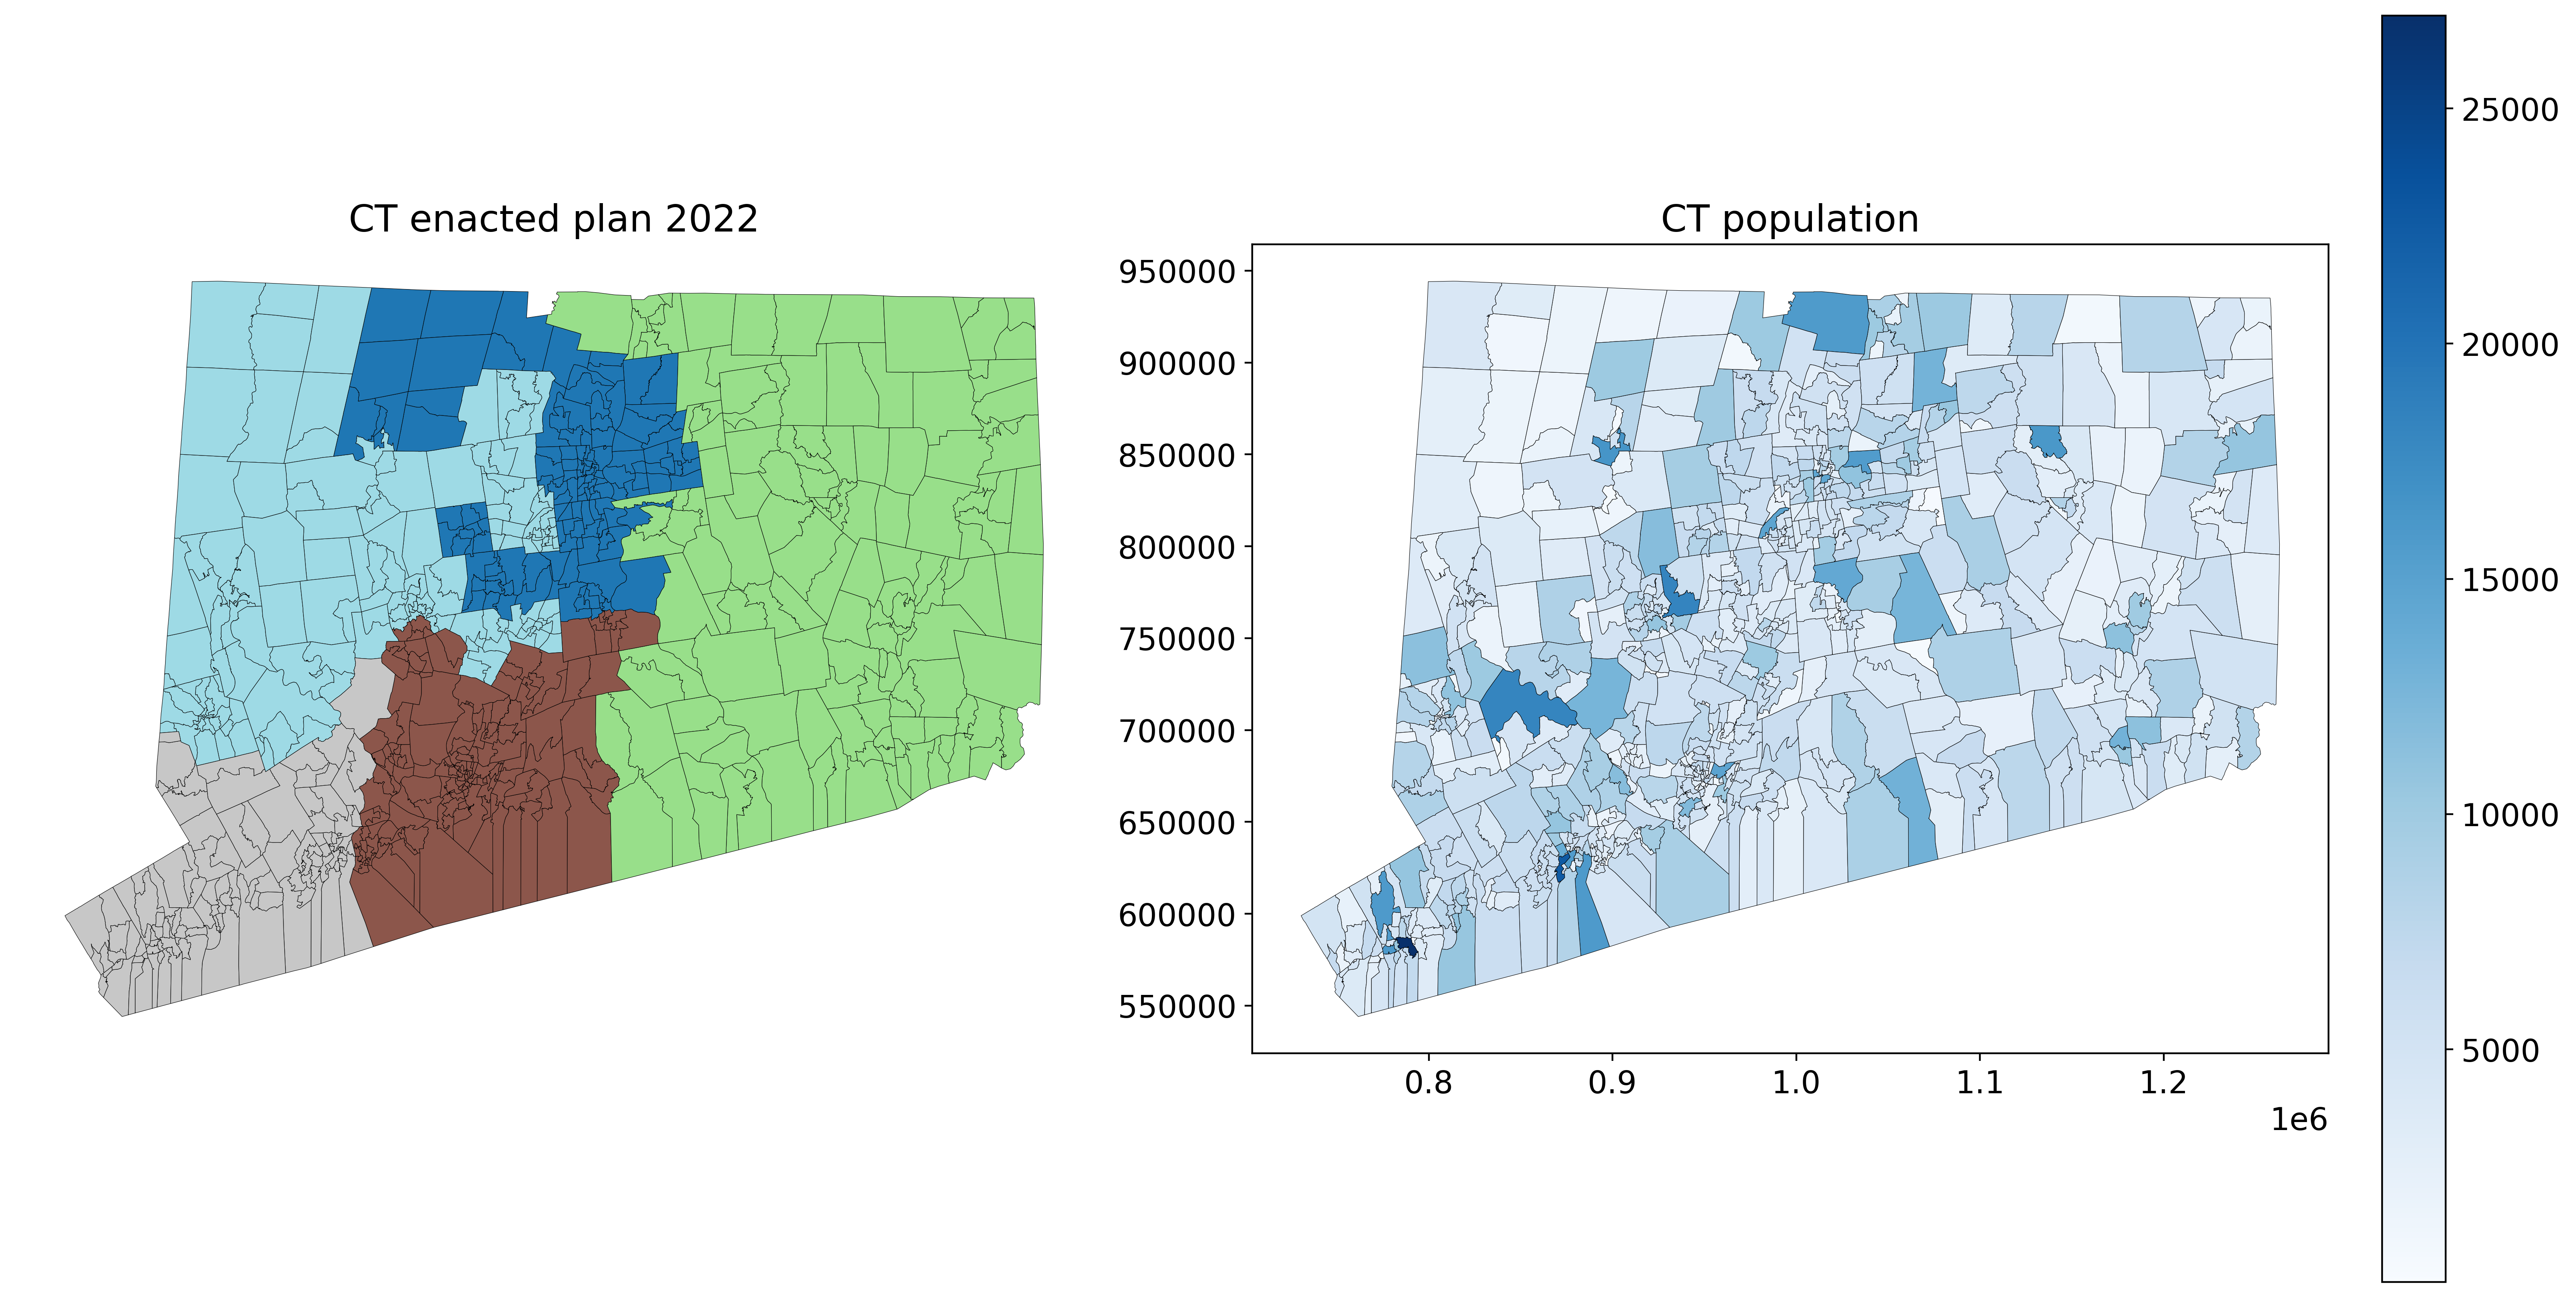
\includegraphics[width=1.0\linewidth]{figures/ct_enacted_pop.png}
    \caption{Population distribution for the enacted Connecticut plan.}
    \label{fig:ct_enacted_pop}
\end{figure}
We work with a $50$K-sample CycleWalk run with $\gamma=0$ (i.e., the tree-count measure).
We notice a clear ``elbow'' in the CT case, where dispersion drops sharply around $K=34$ as shown in Figure \ref{fig:ct_elbow}.
\begin{figure}[!htbp]
    \centering
    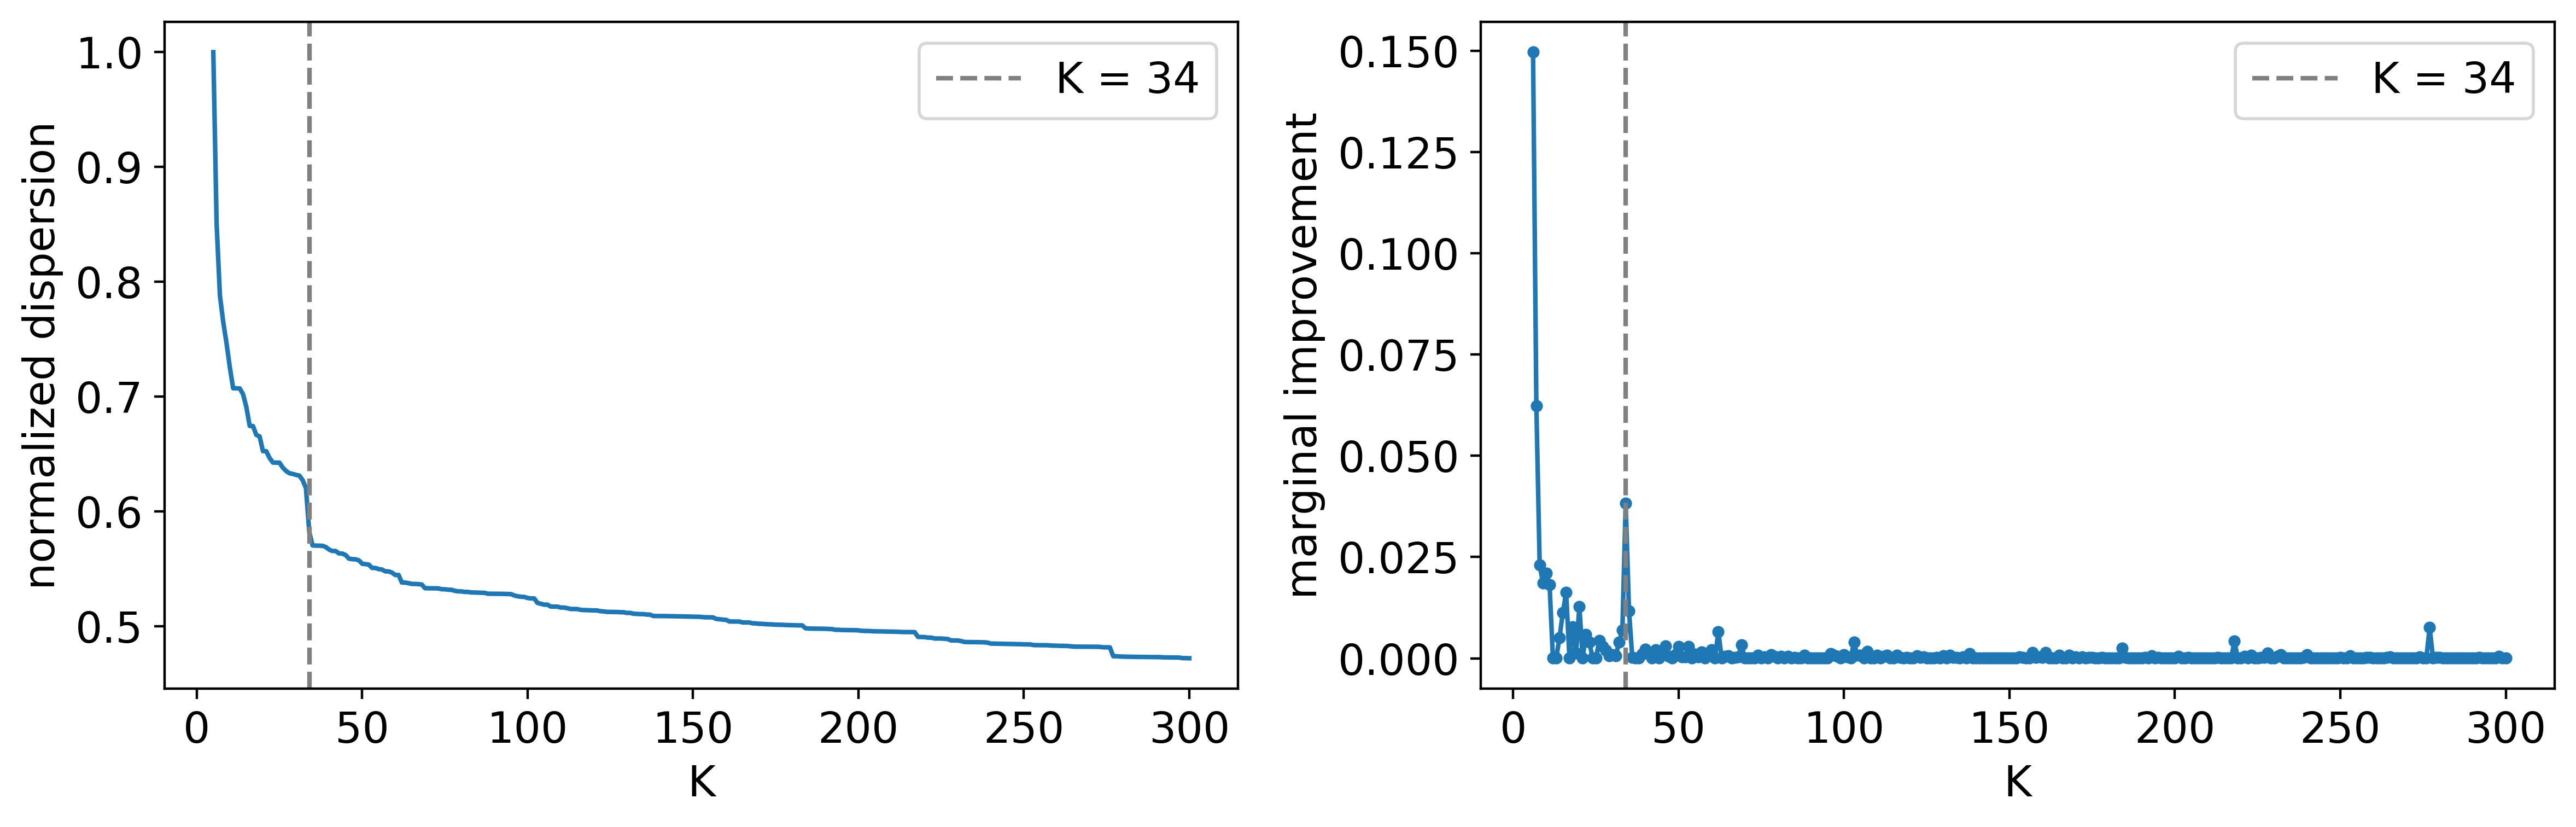
\includegraphics[width=1.0\linewidth]{figures/ct_elbow.png}
    \caption{Elbow plots for CT: left, dispersion metric against number of clusters; right, marginal improvements in the dispersion metric by taking consecutive differences. Dispersion shown is normalized by the first value when $K=5$.}
    \label{fig:ct_elbow}
\end{figure}
Figure \ref{fig:ct_merge_34} shows that the merge of two southwestern clusters corresponds to the sharp drop in dispersion, suggesting an optimal alphabet size of $K=34$.
\begin{figure}[!htbp]
    \centering
    \includegraphics[width=1.0\linewidth]{figures/ct_merge_34.png}
    \caption{Merges of \hccultra around the elbow. Each row shows two child clusters and their merged cluster for a nearby value of $K$. We annotate each merge by the sizes of the clusters involved, as well as the improvement in the dispersion objective. The color on a precinct $p$ indicates the fraction of districts within a cluster that contains $p$.}
    \label{fig:ct_merge_34}
\end{figure}
For the word-level analyses below, we use a slightly finer alphabet with $K=50$ and choose a large beam search width of $L=2000$ to capture the relevant words.
Figure~\ref{fig:ct_top5_word_before_prune} visualizes the five words with the largest observed plan coverage before pruning; several of these high-coverage words are near-duplicates that differ only by small local letter substitutions.
\begin{figure}[!htbp]
    \centering
    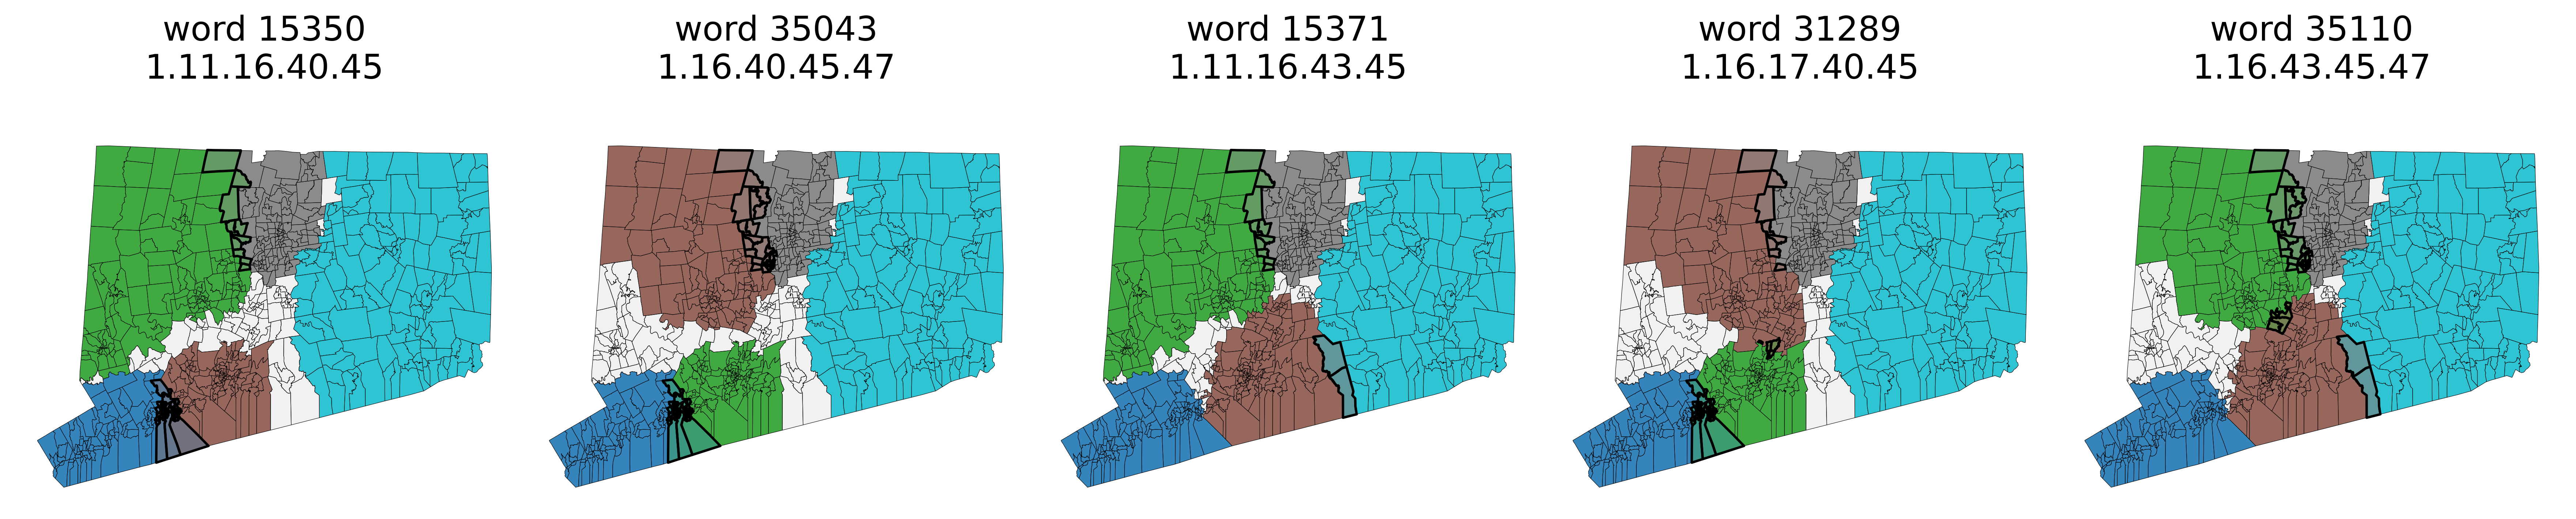
\includegraphics[width=1.0\linewidth]{figures/ct_top5_word_before_prune.png}
    \caption{Top five words (by number of plans covered) before pruning. We visualize words by plotting the letters with different colors. Intersections between letters are highlighted in black lines.}
    \label{fig:ct_top5_word_before_prune}
\end{figure}

To improve interpretability and reduce redundancy while preserving coverage of the observed plans, we construct the pruned set $\mathcal{S}_\eta$ using the two-stage greedy subcover in Algorithm~\ref{alg:eta_greedy_subcover}.
Here we take $\eta=1.0$, which selects $50$ representative words and covers all $49{,}961$ processed plans.
Figure~\ref{fig:ct_top5_word_after_prune} shows that, after pruning, the top words are more diverse and correspond to distinct large-scale plan motifs rather than minor variations within the same mode.
Word $15350$ has the largest coverage and appears in both Figure~\ref{fig:ct_top5_word_before_prune} and Figure~\ref{fig:ct_top5_word_after_prune}; it is selected first in the initial greedy subcover of Algorithm~\ref{alg:eta_greedy_subcover}.
This word is also close to the $2022$ enacted plan.
The southwestern letter (in blue) remains a strong district-level motif after pruning, while the other four districts show more variation across the retained words.

\begin{figure}[!htbp]
    \centering
    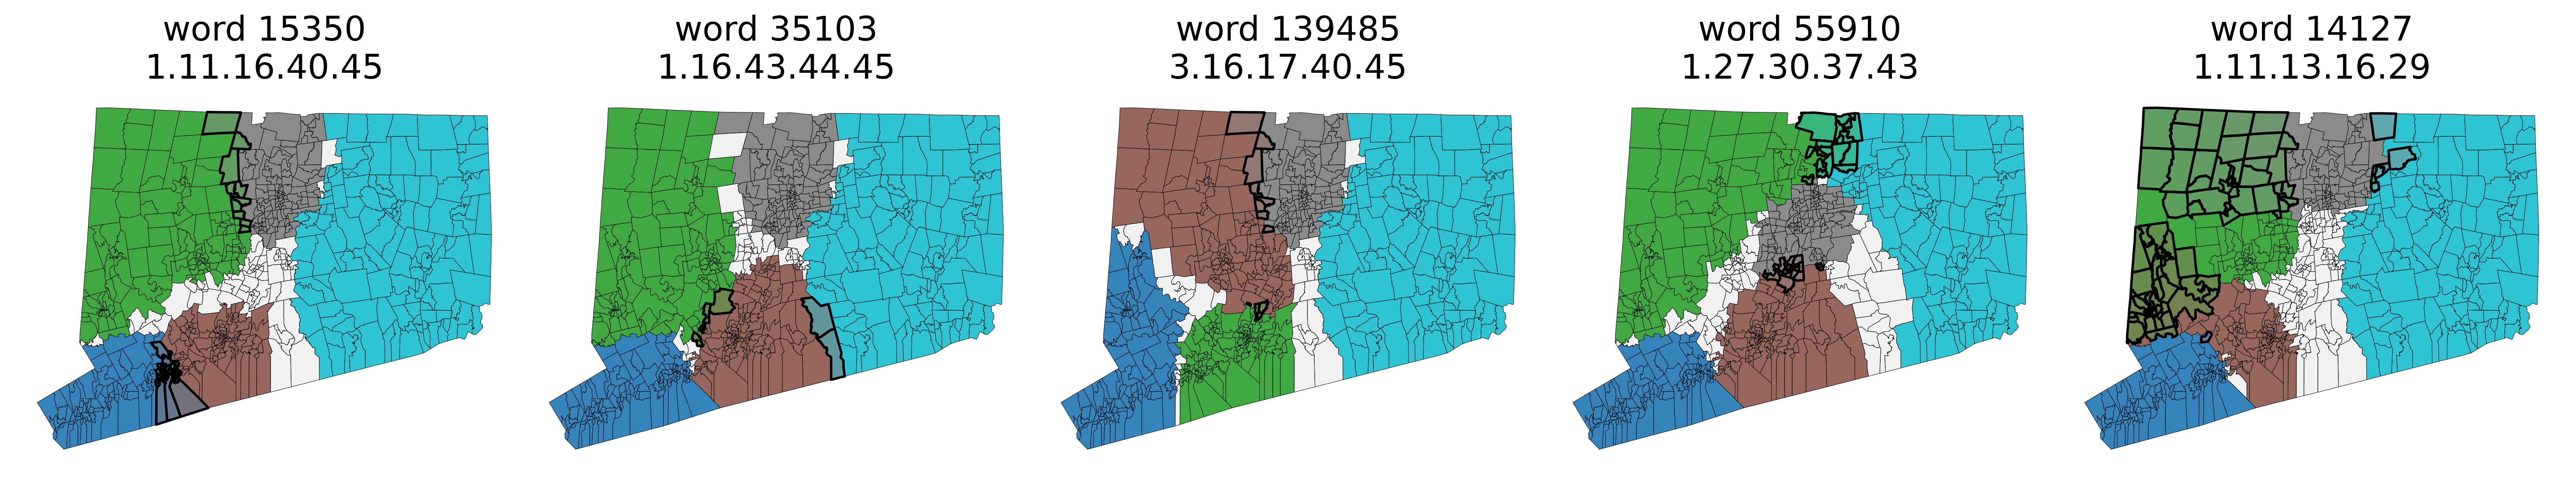
\includegraphics[width=1.0\linewidth]{figures/ct_top5_word_after_prune.png}
    \caption{Similar to Figure \ref{fig:ct_top5_word_before_prune} but for the pruned set $\mathcal{S}_\eta$ produced by the two-stage greedy subcover. Pruning removes near-duplicate strata while maintaining coverage of the sampled ensemble, yielding a more compact and interpretable set of representative words.}
    \label{fig:ct_top5_word_after_prune}
\end{figure}

It is also interesting to see how the enacted plan fits into our strata, even though it follows a quite different measure.
In practice, redistricting plans are typically proposed by legislators and accepted through a political process.
See Figure \ref{fig:ct_enacted_words} for a visualization of the nearest words to the $2022$ enacted plan.
We compare the three closest words before pruning and in the two-stage pruned set $\mathcal{S}_\eta$.
As expected, the minimum distance between the enacted plan and the representative word set increases after pruning, from about $1.34$M to $1.47$M in the displayed distance.
Nevertheless, the closest word in the pruned word set successfully captures the macroscopic spatial structure of the plan.
Note that we do not see any highly specific local boundary geometry even before pruning, e.g. the dark blue district in the north-central region of the enacted plan.
These localized features are intentionally smoothed out during the hierarchical clustering phase, which abstracts districts into representative letters.
\begin{figure}[!htbp]
    \centering
    \includegraphics[width=1.0\linewidth]{figures/ct_enacted_words.png}
    \caption{Closest words to the enacted plan. The first and second rows of the $2\times 3$ word plots show the three closest words after and before pruning, respectively. For each word displayed, we annotate its distance to the enacted plan.}
    \label{fig:ct_enacted_words}
\end{figure}

Next, we compute stationary distributions using multiple choices of temperatures while keeping the range mapping function $\kappa$ fixed.
Typically, we could tune $T$ and $\kappa$ based on empirical observations from stratified sampling.
Since we do not implement stratified sampling in the current paper, we pick a generic $\kappa$ that maps most of the pruned nearest neighbors into the $[0,1]$ range (and zero if a word is not within beam width).
We vary the temperature over $T=0,10,20$ in Figure \ref{fig:ct_stat_flux}.
Specifically, we include the case of $T=0$ (the counting measure) as an example that is $\kappa$ independent.
\begin{figure}[!htbp]
    \centering
    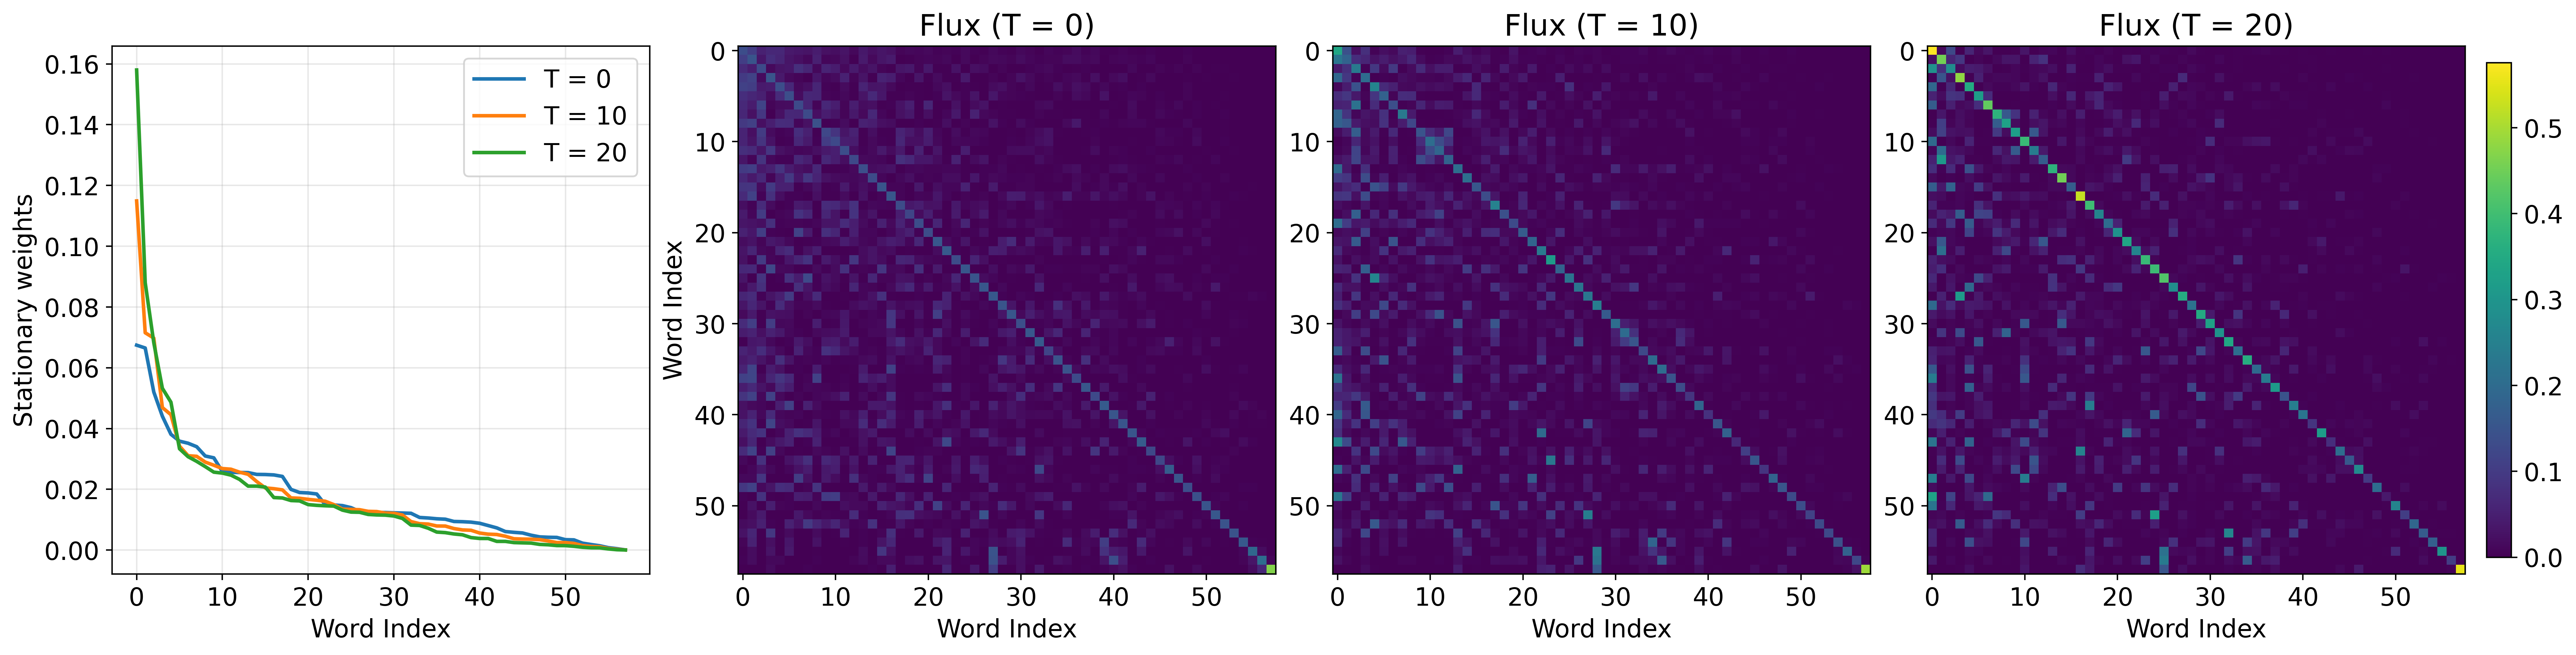
\includegraphics[width=1.0\linewidth]{figures/ct_stat_flux.png}
    \caption{Stratum weights and flux matrices for $T=0,10,20$.}
    \label{fig:ct_stat_flux}
\end{figure}
At the intermediate temperature $T=10$, we see reasonable overlaps across most strata except for the smallest one, which corresponds to an atypical plan.
See Figure \ref{fig:ct_top_bot_words} for more details, where we illustrate the three largest and three smallest strata together with example plans attached to those words.
\begin{figure}[!htbp]
    \centering
    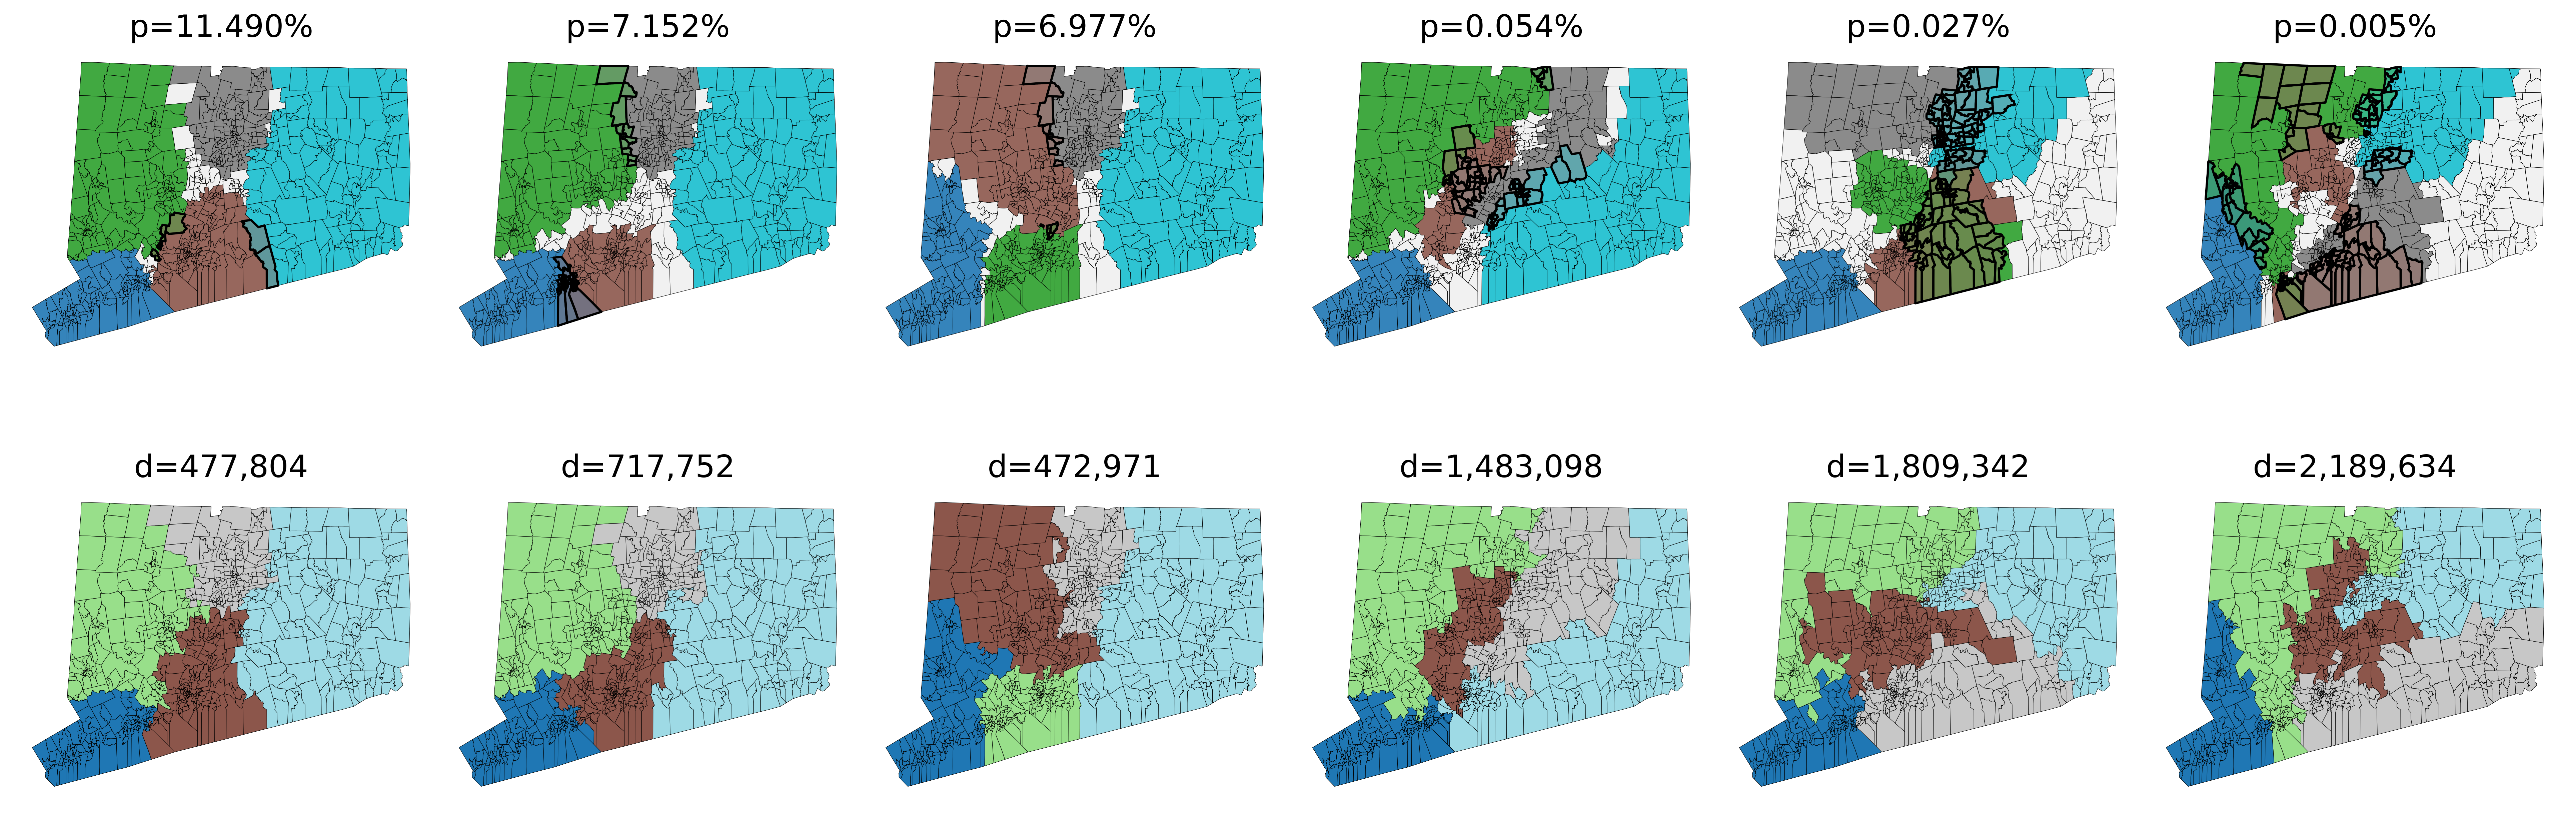
\includegraphics[width=1.0\linewidth]{figures/ct_top_bot_words.png}
    \caption{Top and bottom three words according to the stationary distribution at $T=10$. Words are shown in the first row, and example plans attached to those words are shown in the second row.}
    \label{fig:ct_top_bot_words}
\end{figure}


\subsection{Beyond $\gamma=0$}
In this section, we study how our strata construction generalizes to other $\gamma$.
Same as~\cite{cyclewalk}, we sample from a family of unnormalized probability distributions proportional to $\exp\{-\gamma J_{\mathrm{tree}}(x)-c_\gamma J_{\mathrm{iso}}(x)\}$ parametrized by $(\gamma,c_\gamma)$, where $J_{\mathrm{tree}}$ is the log spanning-forest count and $J_{\mathrm{iso}}$ is the sum of district isoperimetric scores.
We refer to $c_\gamma$ as the iso parameter.
Intuitively, larger iso parameters tilt the target distribution toward smaller isoperimetric scores, i.e., more compact districts.
Meanwhile, increasing $\gamma$ from $0$ to $1$ tilts the distribution more toward uniform partitions, which are less compact.

As a first step, we calibrate the iso parameter to obtain, for each $\gamma$ from $0$ to $1$, an iso parameter that produces samples with isoperimetric ratio comparable to that of $(0,0)$.
We see that the relationship between $\gamma$s and calibrated iso parameters is roughly linear, which is consistent with the observations in~\cite{cyclewalk}.
See Figure~\ref{fig:iso_calibration} for more details.
After calibration, the isoperimetric-score distributions remain comparable across $\gamma$, while the distribution of log spanning-forest counts shifts downward as $\gamma$ increases.
Keeping compactness comparable makes it more reasonable to use strata constructed from one distribution to study another distribution in this family.
\begin{figure}[!htbp]
    \centering
    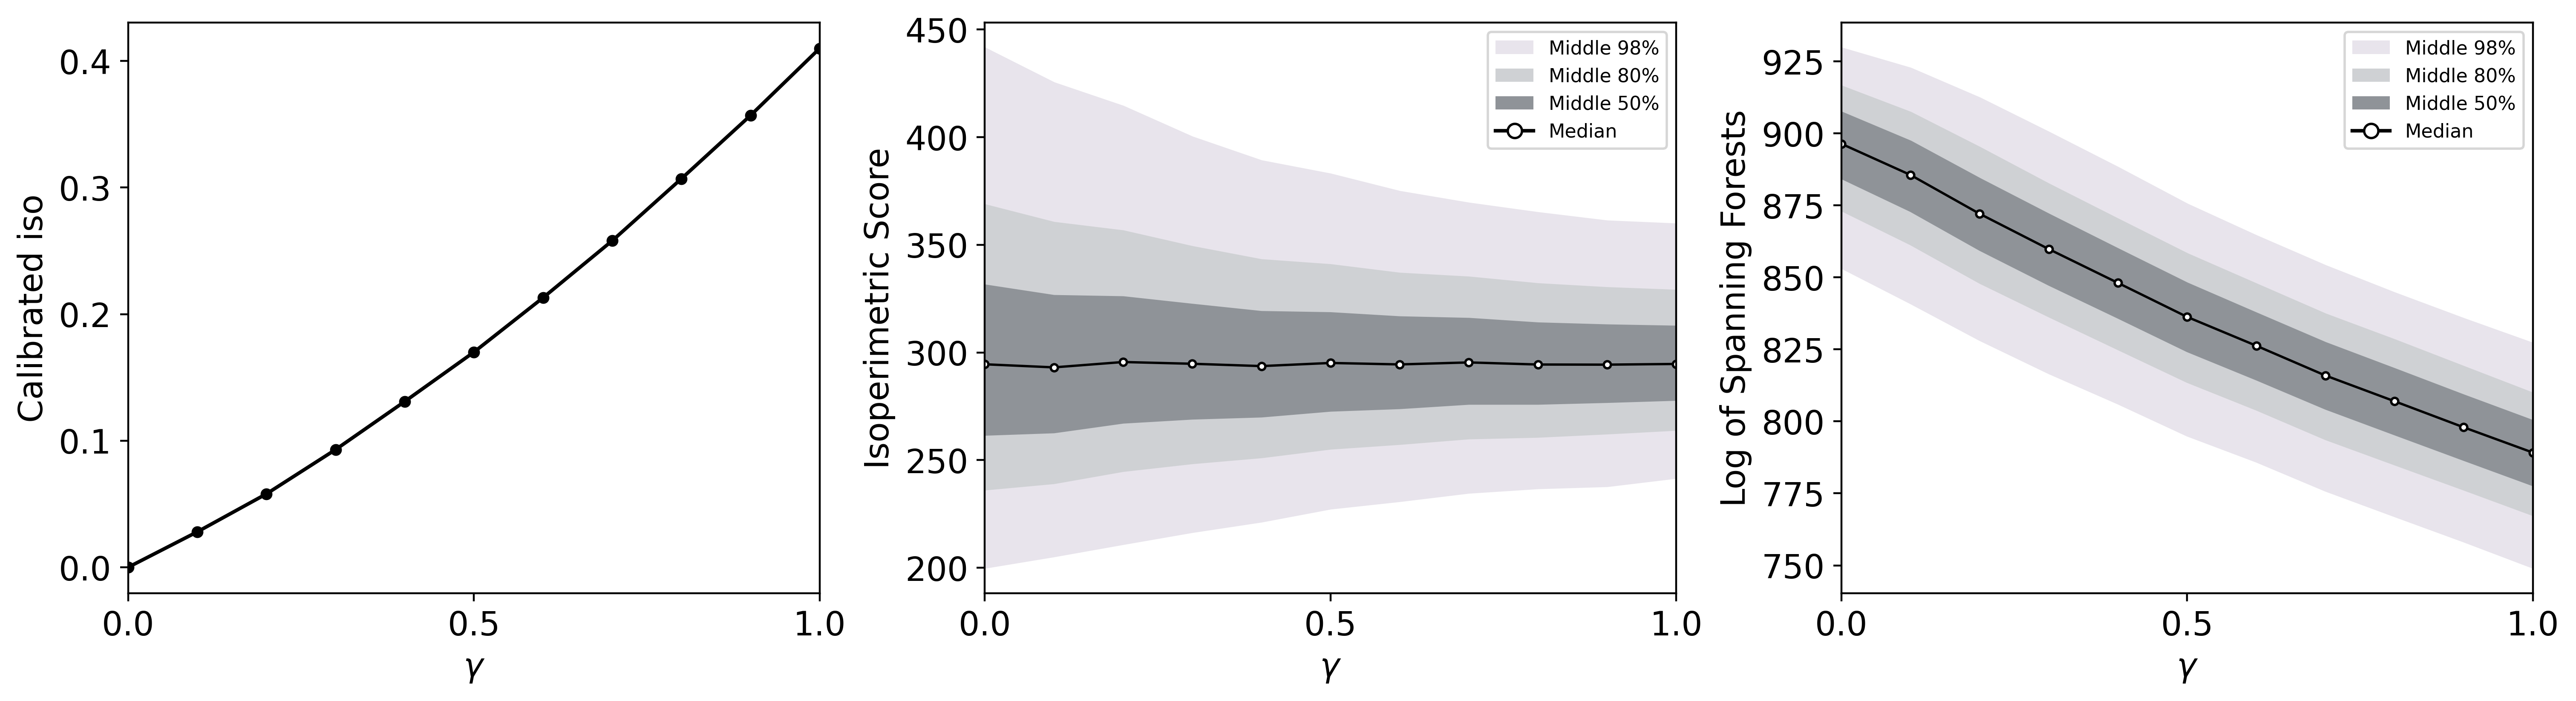
\includegraphics[width=1.0\linewidth]{figures/iso_calibration.png}
    \caption{Calibration of the isoperimetric parameter for target measures indexed by $\gamma$. Left: calibrated iso value for each $\gamma$. Middle: isoperimetric-score distributions, with shaded bands showing the middle $50\%$, $80\%$, and $98\%$ intervals and markers showing medians. Right: distributions of log spanning-forest counts.}
    \label{fig:iso_calibration}
\end{figure}
Figure~\ref{fig:ct_cmds_overlay_seed_A} gives a geometric view of how the sampled district distribution changes as $\gamma$ varies.
To produce this visualization, we compute pairwise weighted $\ell^1$ distances between districts sampled from the three target distributions and project them to two dimensions using classical multidimensional scaling~\cite{torgerson1952multidimensional}.
The three point clouds occupy a common low-dimensional geometry, but their mass shifts as $\gamma$ changes.
This suggests that the alphabet computed with $\gamma=0$, shown as black diamonds in Figure \ref{fig:ct_cmds_overlay_seed_A}, remains informative for other target distributions in this family, while becoming less centered on the target distribution as $\gamma$ moves away from $0$.
\begin{figure}[!htbp]
    \centering
    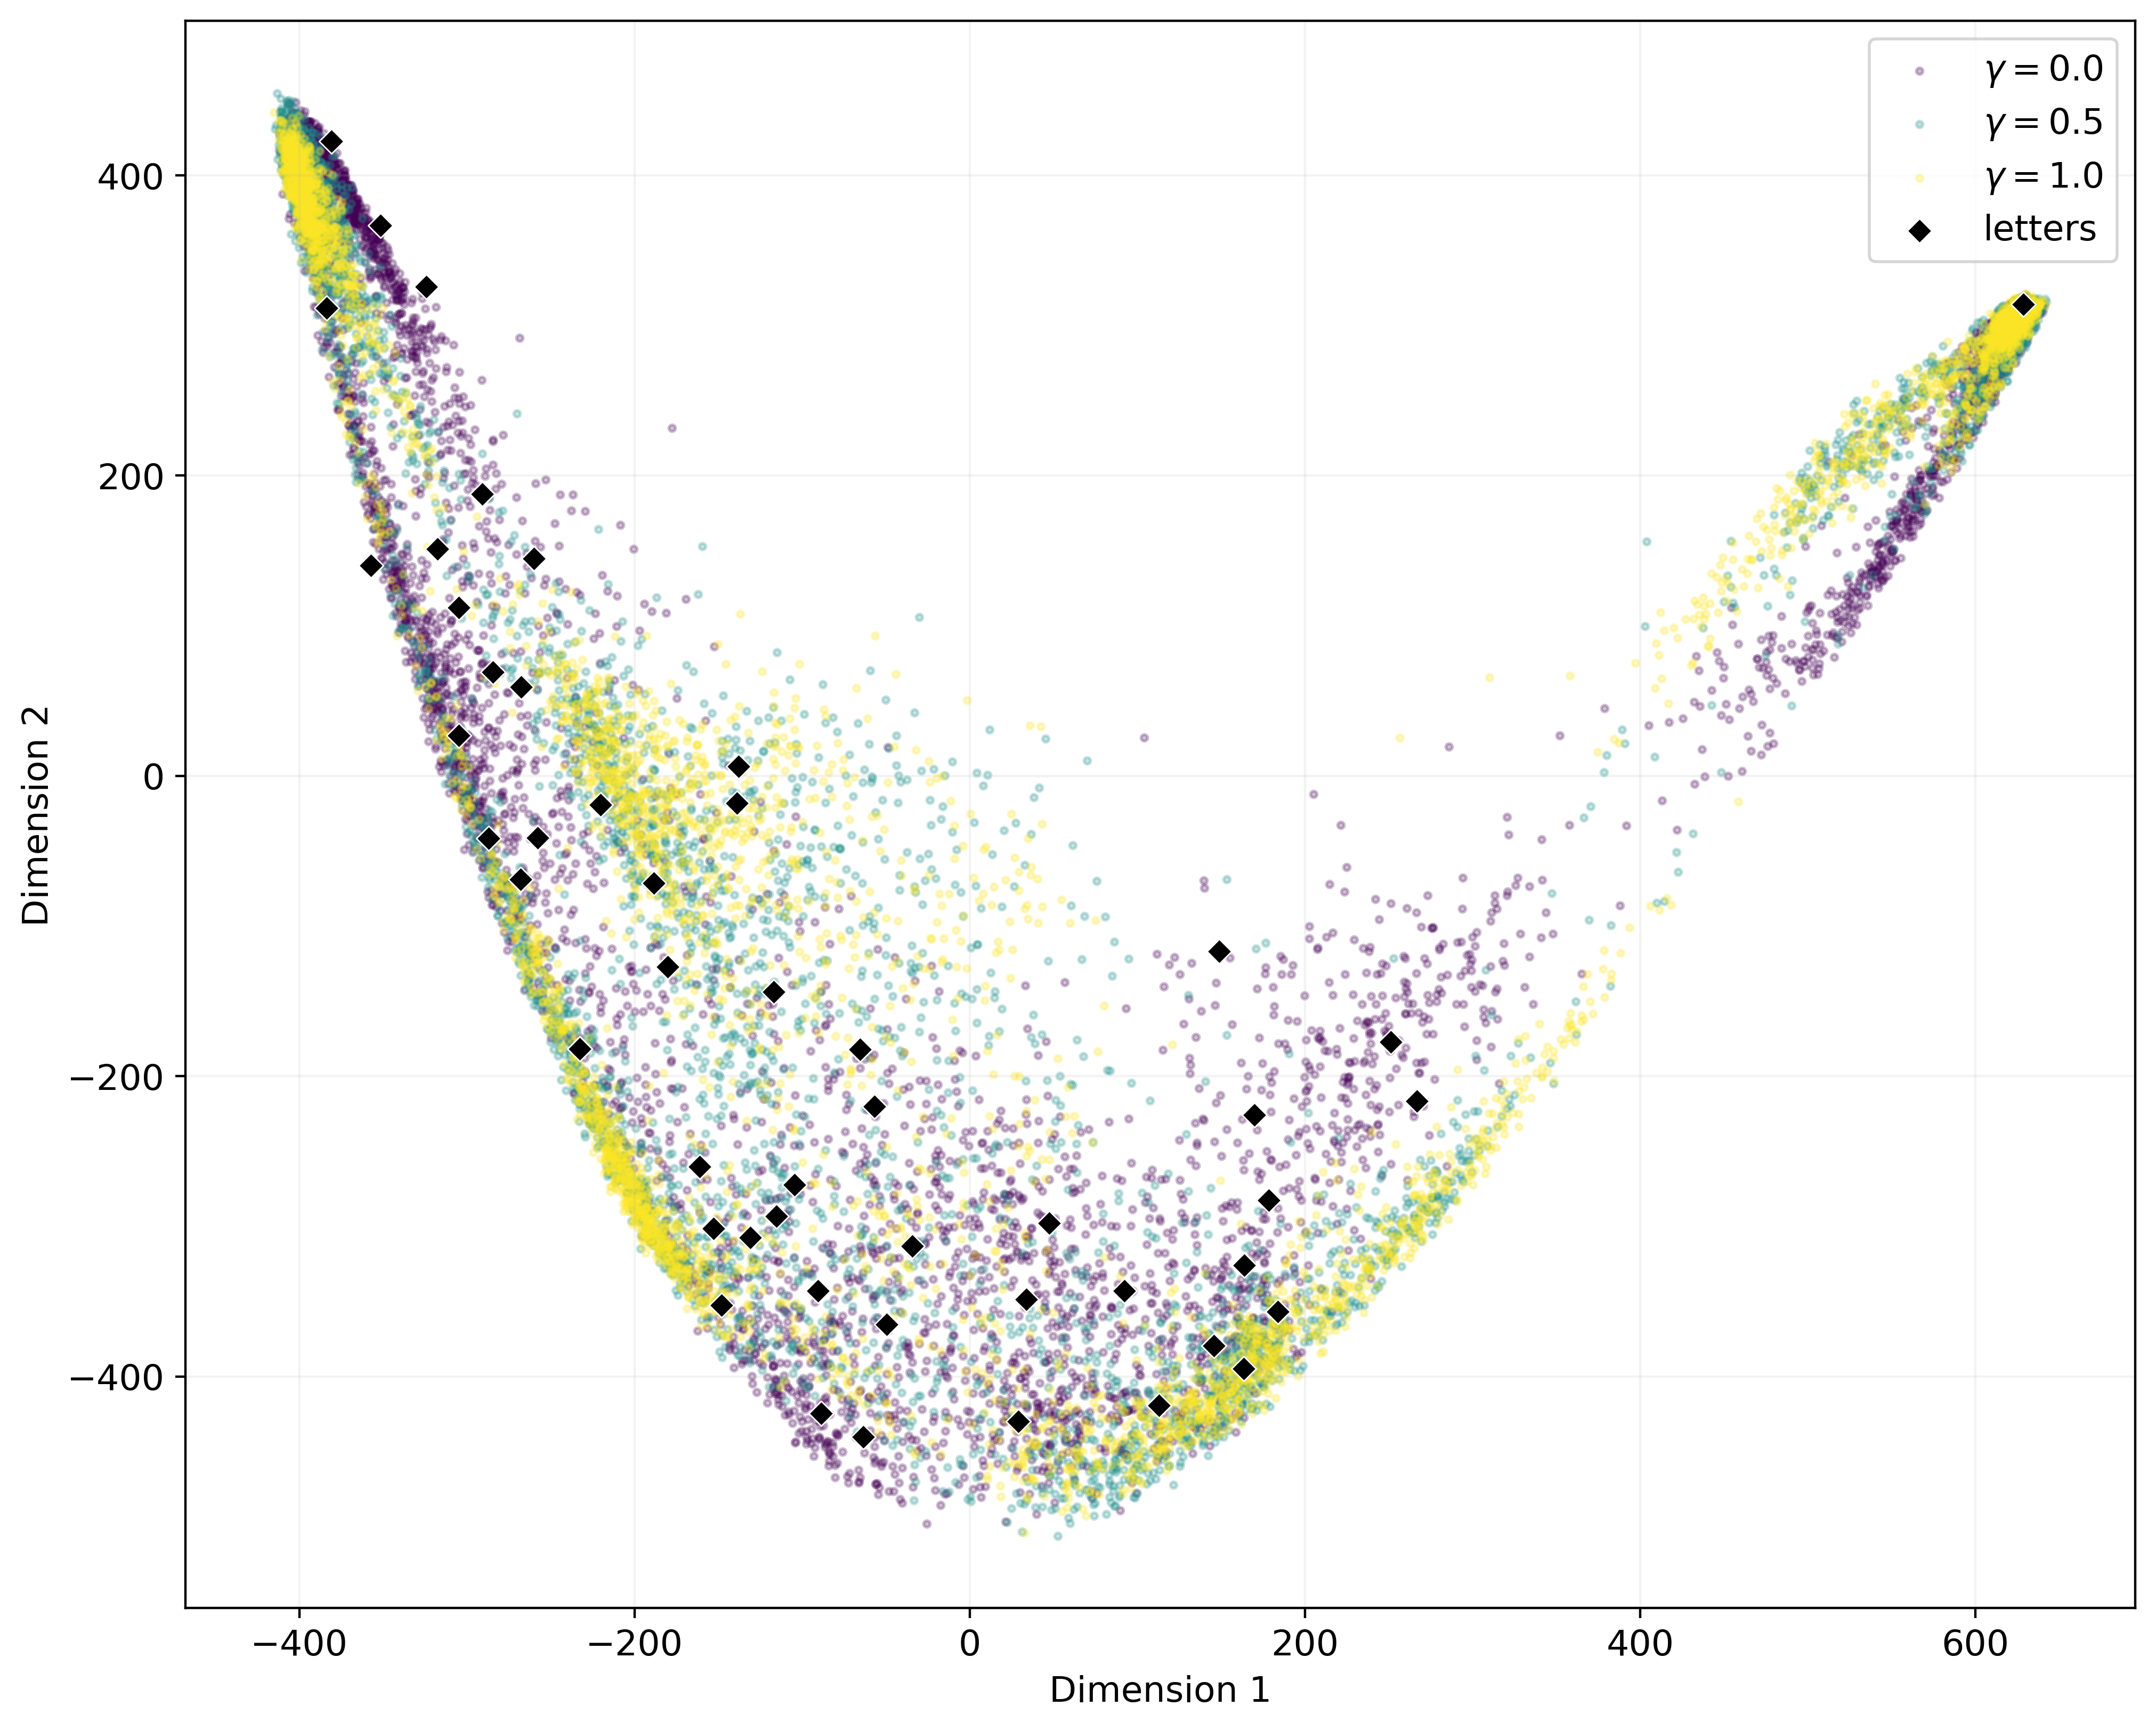
\includegraphics[width=0.92\linewidth]{figures/ct_cmds_overlay_0p0_0p5_1p0_seed_A.png}
    \caption{Classical multidimensional scaling embedding of Connecticut sampled districts for $\gamma\in\{0,0.5,1.0\}$ using seed A. Colors indicate $\gamma$, and black diamonds denote the representative letters learned from the baseline ensemble.}
    \label{fig:ct_cmds_overlay_seed_A}
\end{figure}

In practice, we would like to construct strata using samples from $\gamma=0$, where sampling is relatively cheap, and then use those strata to study other values of $\gamma$.
For this to be reasonable, the resulting words should still have enough overlap under the other target distributions.
As a first sanity check, we fix $\eta=0.70$ and $T=10$ and repeat the computation with two independent runs.
Figure~\ref{fig:ct_gamma_eta_0.70_T_10} shows that the qualitative spectral-gap behavior is consistent across seeds.
The differences between the two flux matrices and stationary distributions grow for larger $\gamma$, which may reflect slower convergence of the underlying chains as the target moves farther from the tree-count measure.
For other combinations of $\eta$ and $T$, we see patterns that are qualitatively similar.
\begin{figure}[!htbp]
    \centering
    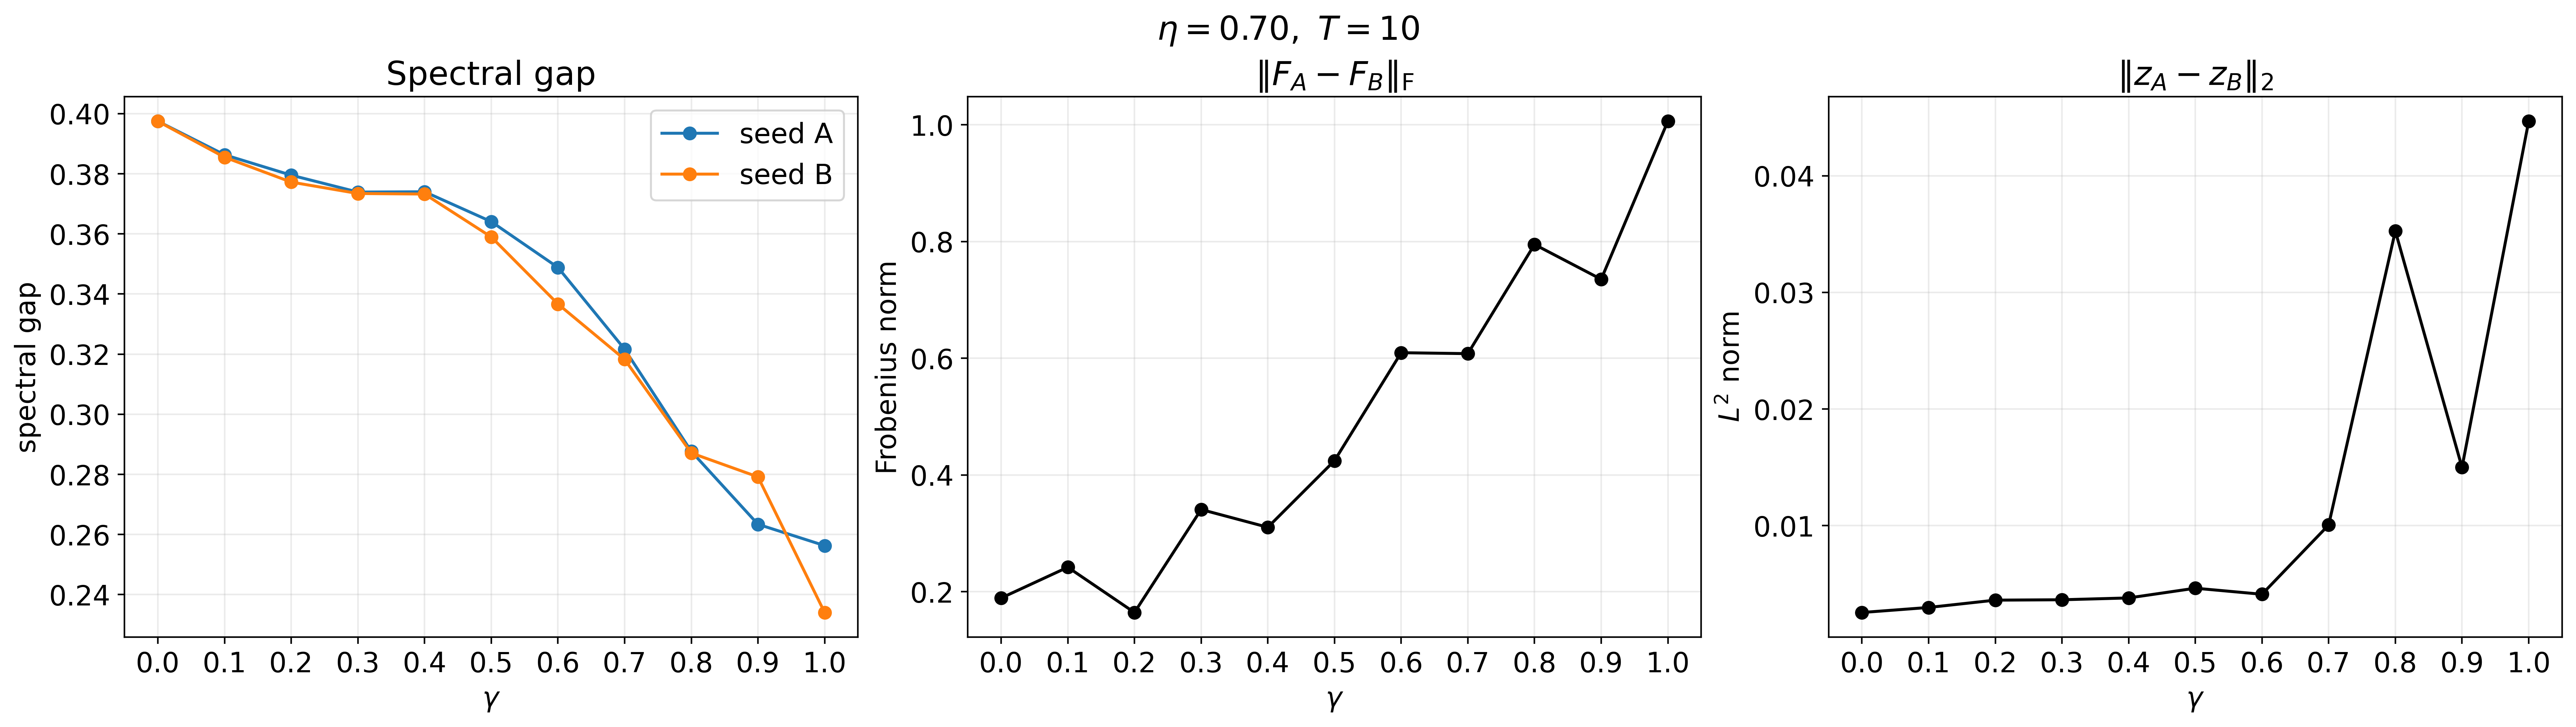
\includegraphics[width=1.0\linewidth]{figures/ct_gamma_eta_0.70_T_10.png}
    \caption{Comparison of two independent runs as $\gamma$ varies, with $\eta=0.70$ and $T=10$. Left: spectral gap of the flux matrix $F$ in \eqref{eq:flux}. Middle: Frobenius norm $\|F_A-F_B\|_F$. Right: $\ell^2$ distance $\|z_A-z_B\|_2$ between the stationary distributions.}
    \label{fig:ct_gamma_eta_0.70_T_10}
\end{figure}
\FloatBarrier

We then examine how the POU temperature and pruning threshold affect this diagnostic.
We select threshold parameters $\eta=0.59,0.63,0.70$, which produce word sets of sizes $188,103,50$, respectively, and compute flux matrices for temperatures $T=0,10,20$.
Together, these choices give nine experimental configurations.
Figure~\ref{fig:ct_gamma_spectral_gap_seed_A_by_temperature} shows the spectral gap of the resulting flux matrices as $\gamma$ varies.
The spectral gap decreases for two related reasons: larger $\gamma$ moves the target distribution away from the $\gamma=0$ distribution used to construct the strata, while larger $T$ concentrates each word on closer plans and therefore reduces its effective support.
\begin{figure}[!htbp]
    \centering
    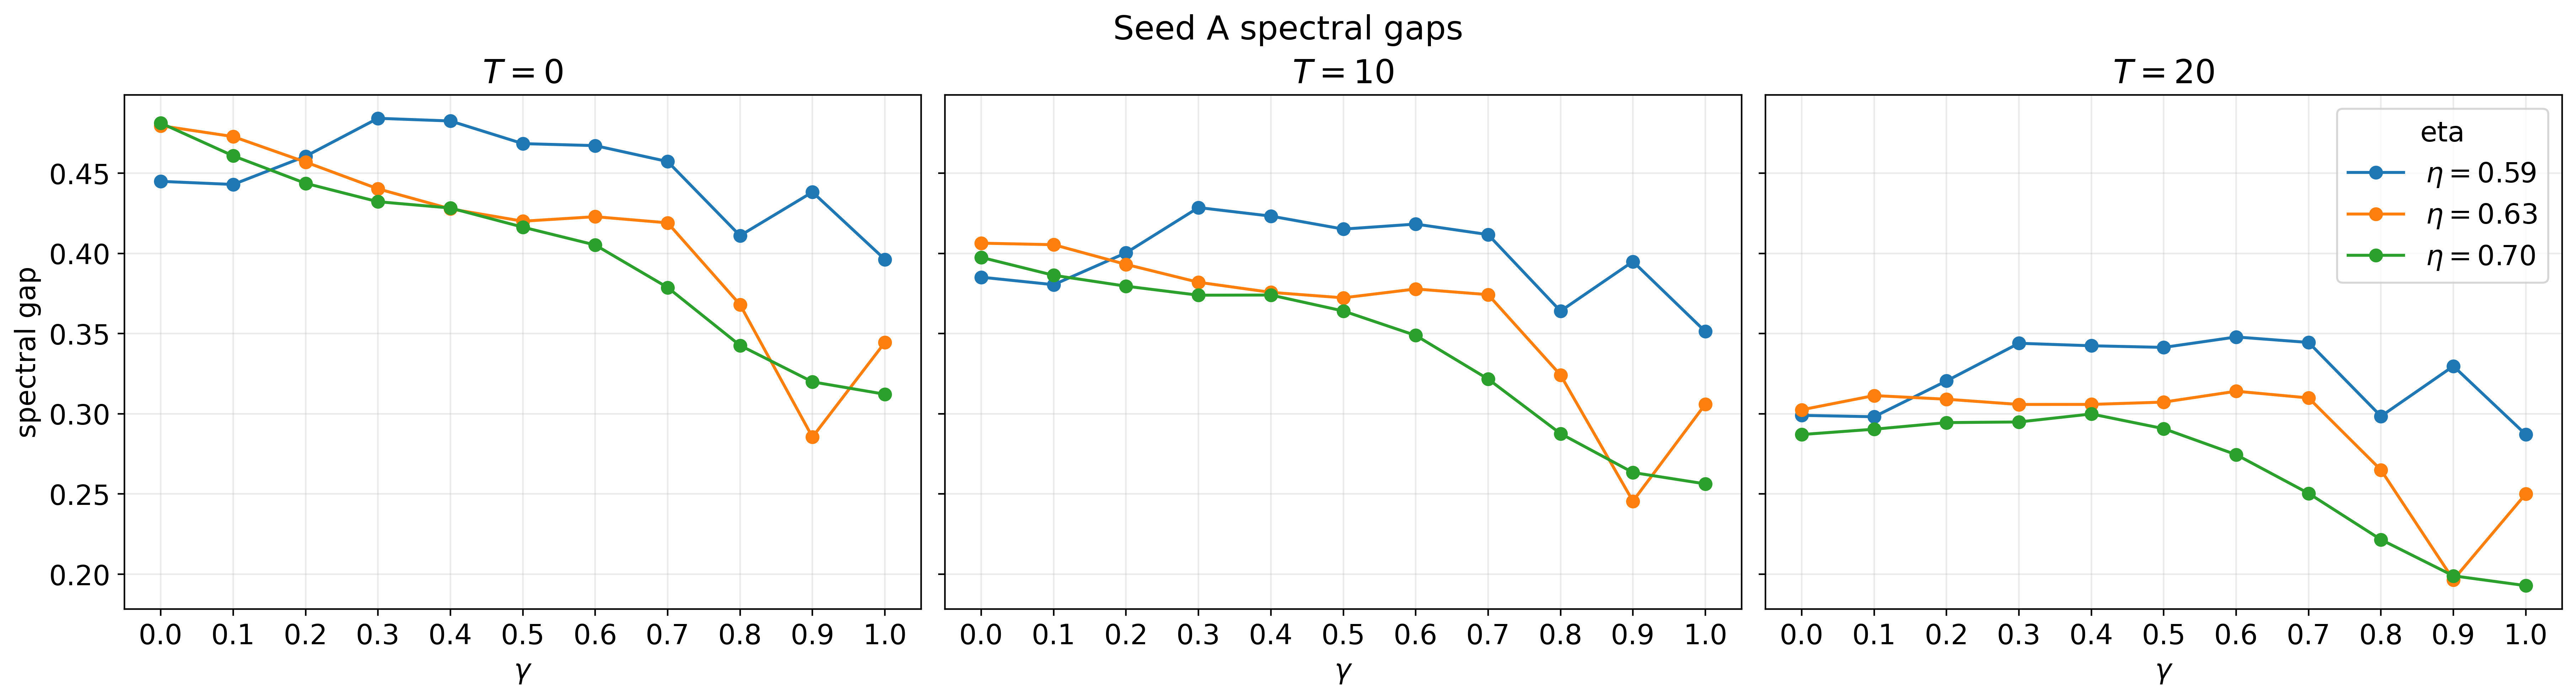
\includegraphics[width=1.0\linewidth]{figures/ct_gamma_spectral_gap_seed_A_by_temperature.png}
    \caption{Spectral gap of the flux matrix $F$ in \eqref{eq:flux} for seed A as $\gamma$ varies. Each panel fixes the temperature $T$ in the POU kernel \eqref{eq:psi_relative}, while colors indicate the threshold parameter $\eta$ used in Algorithm~\ref{alg:eta_greedy_subcover}.}
    \label{fig:ct_gamma_spectral_gap_seed_A_by_temperature}
\end{figure}

% internal comment: we have nc results but it's incomplete so i don't plan to include it
% \subsection{North Carolina}\label{sec:north_carolina}
% We next apply the pipeline to redistricting plans of North Carolina, where $|V|=2671$ precincts are partitioned into $I=14$ congressional districts.
% In the NC case, the elbow appears at a larger $K$ due to the increase in the number of districts.
% We see that the dispersion drops sharply around $K=129$, as shown in Figure~\ref{fig:nc_elbow}.
% \begin{figure}[!htbp]
%     \centering
%     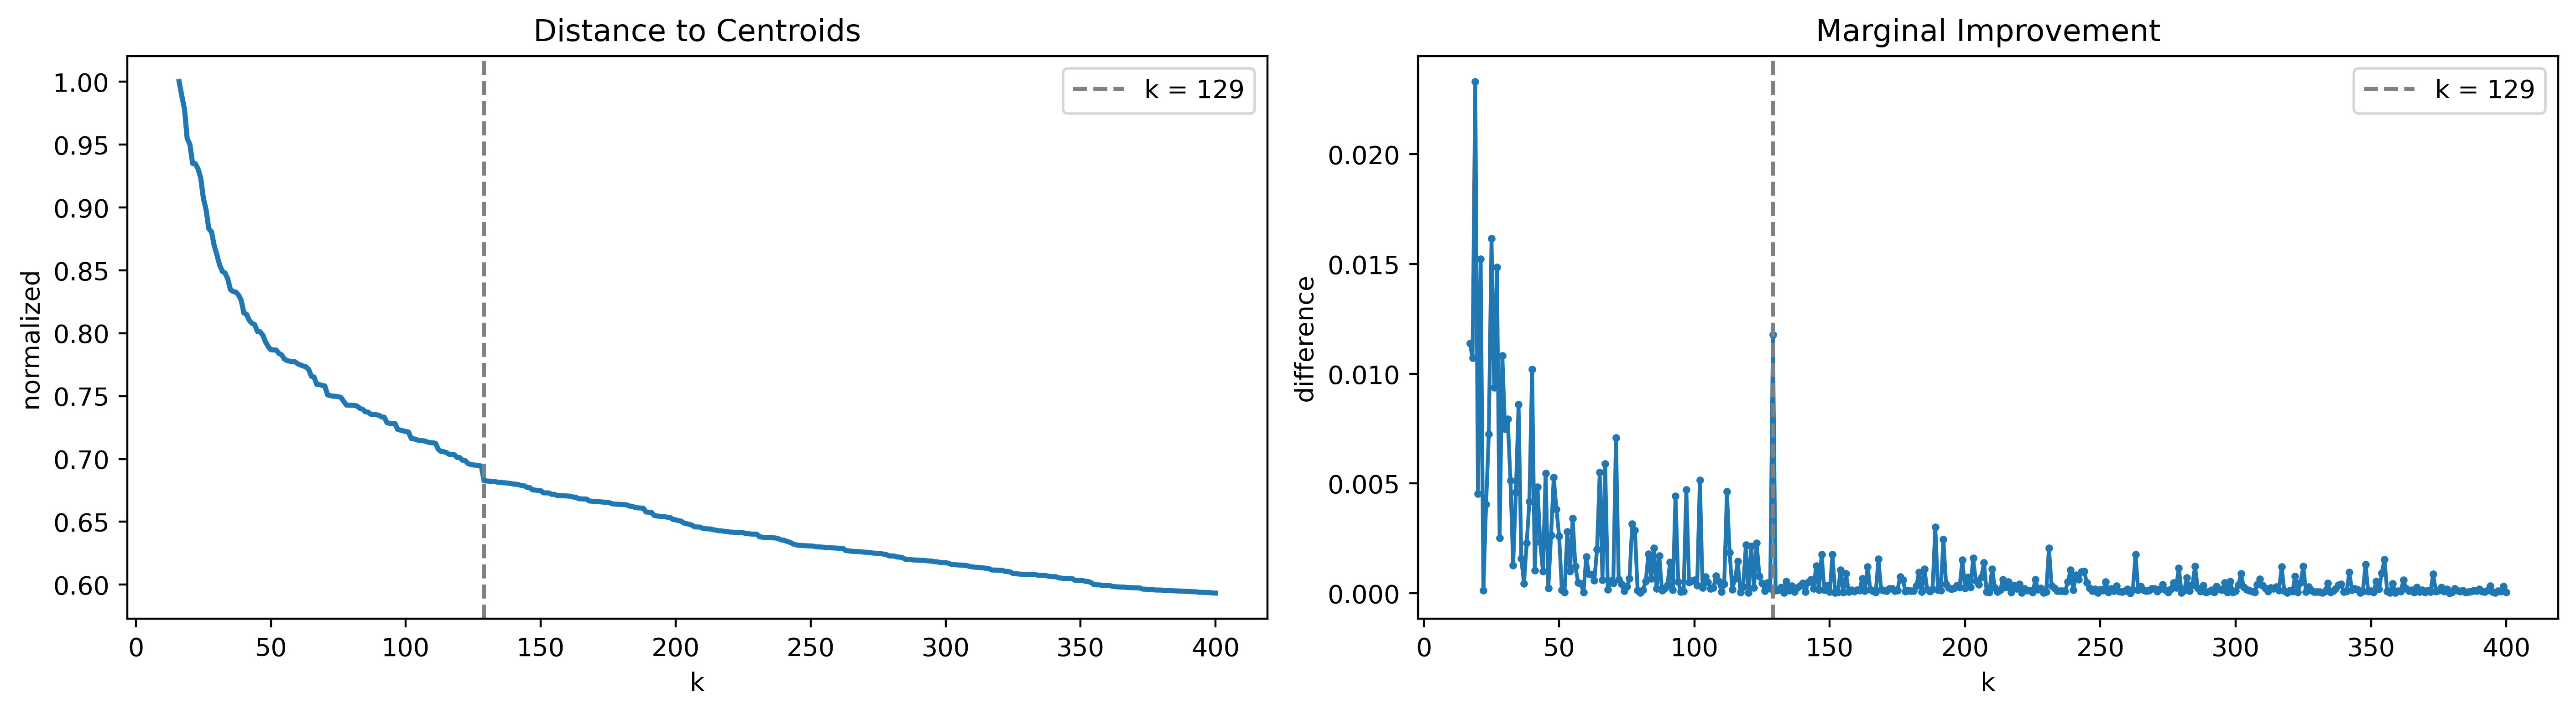
\includegraphics[width=1.0\linewidth]{figures/nc_elbow.png}
%     \caption{Elbow plots for NC - left: dispersion metric against number of clusters, right: marginal improvements on the dispersion metric by taking consecutive differences.}
%     \label{fig:nc_elbow}
% \end{figure}
% Figure~\ref{fig:nc_merge_129} visualizes the \hccultra merges around this elbow, suggesting an optimal alphabet size around $K=129$.
% \begin{figure}[!htbp]
%     \centering
%     \includegraphics[width=1.0\linewidth]{figures/nc_merge_129.png}
%     \caption{The merges of \hccultra around the elbow in the NC case. Each row represents a merge performed by \hccultra of two clusters into one (indicated by left, right and merged). The color on a precinct $p$ indicates the fraction of districts within a cluster that contains $p$.}
%     \label{fig:nc_merge_129}
% \end{figure}

% We set an alphabet size of $K=129$ and choose a big enough beam search width of $L=1000$ to capture all relevant words.
% Figure~\ref{fig:nc_top5_word_before_prune} visualizes the five words with the largest estimated stratum weights before pruning; as in the CT case, several of these high-weight words are near-duplicates that differ only by small local letter substitutions.
% \begin{figure}[!htbp]
%     \centering
%     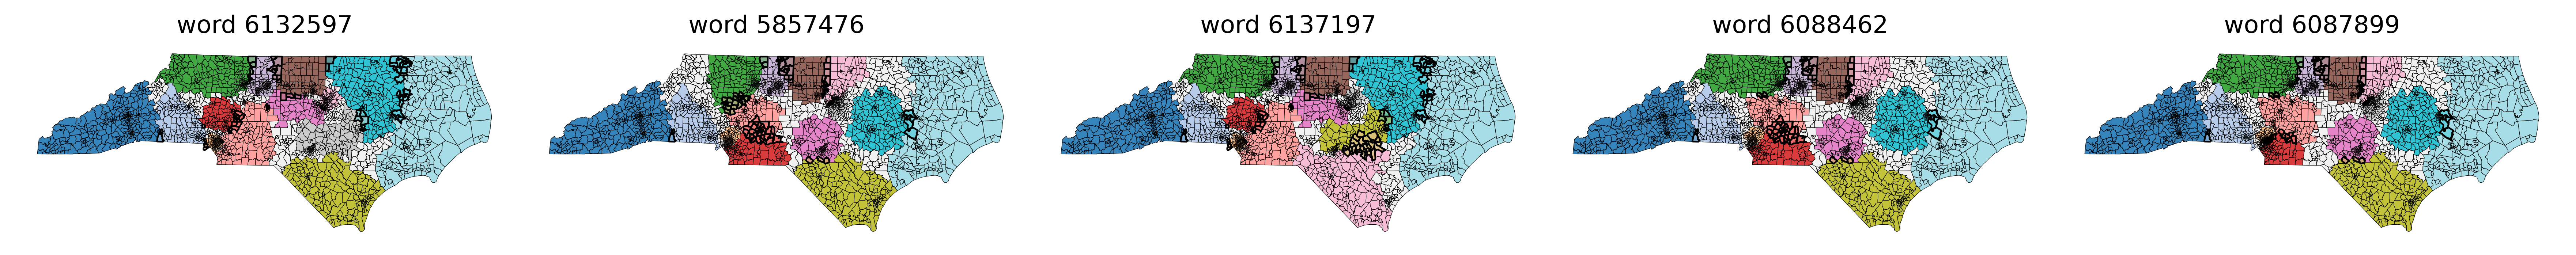
\includegraphics[width=1.0\linewidth]{figures/nc_top5_word_before_prune.png}
%     \caption{Top five words (by number of plans covered) before pruning. We visualize words by plotting the letters with different colors. Intersections between letters are highlighted in black lines.}
%     \label{fig:nc_top5_word_before_prune}
% \end{figure}

% We again construct the pruned set $\mathcal{S}_\eta$ using the two-stage greedy subcover in Algorithm~\ref{alg:eta_greedy_subcover}.
% Figure~\ref{fig:nc_top5_word_after_prune} shows that, after pruning, the top words are more diverse and correspond to distinct plan motifs rather than minor variations.
% Word $6132597$ covers most plans, hence appears in both Figure~\ref{fig:nc_top5_word_before_prune} (by definition) and Figure~\ref{fig:nc_top5_word_after_prune} since it is selected first in the initial greedy subcover of Algorithm~\ref{alg:eta_greedy_subcover}.
% \begin{figure}[!htbp]
%     \centering
%     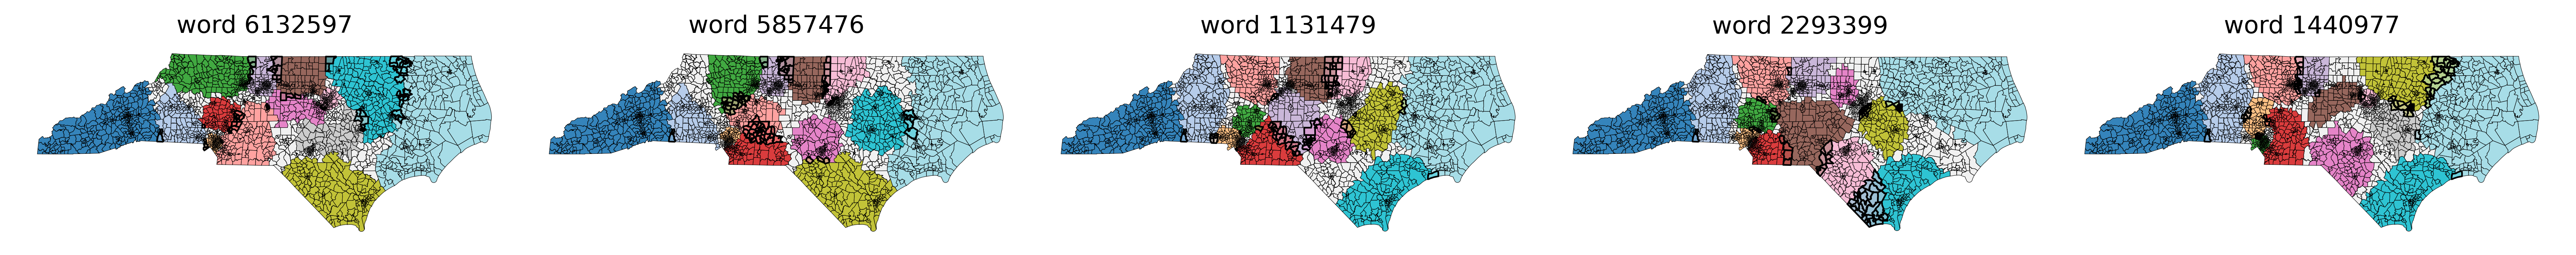
\includegraphics[width=1.0\linewidth]{figures/nc_top5_word_after_prune.png}
%     \caption{Similar to Figure~\ref{fig:nc_top5_word_before_prune} but for the pruned set $\mathcal{S}_\eta$ produced by the two-stage greedy subcover. Pruning removes near-duplicate strata while maintaining coverage of the sampled ensemble, yielding a more compact and interpretable set of representative words.}
%     \label{fig:nc_top5_word_after_prune}
% \end{figure}
% \FloatBarrier

\section{Future Directions}\label{sec:chap4 future_directions}

The natural next step is to use this stratification to run stratified sampling to estimate a plan-level observable of interest $f$, for instance, democratic vote shares.
Let $\pi$ be the target distribution $e^{-J(x)}$ and $\{\phi_s\}_{s\in[S]}$ be the POU that we construct using the pipeline introduced in this paper.
We define the tilted stratum distributions by 
    \begin{align}
        \pi_s(x)\propto e^{-J_s(x)},\quad\quad J_s(x):=J(x)-\phi_s(x).
    \end{align}
Using the same method (e.g. cycle walk), we sample $S$ chains with the biased energy $J_s(x)$.
The Metropolis-Hastings steps need to be adjusted to satisfy detailed balance with respect to the tilted measures $\pi(s)$.
We then apply standard fix-point iterations methods to recover the normalizing factors $z_s$, so that we can estimate $f$ by
    \begin{align}
        \mathbb{E}_\pi[f]:=\sum_{s=1}^Sz_s\mathbb{E}_{\pi_s}[f].
    \end{align}
Ideally, each chain focus on plans around a different word $w_s\in\mathcal{S}$, which allows for more accurate estimates of the observables.

Another interesting direction is to adaptively update the alphabet as we obtain new data, so that the alphabet still captures the motifs in district space.
This can be useful when the original sample used to construct the alphabet is too small, or when the target distribution changes drastically, causing new motifs to appear.
Re-running hierarchical clustering from scratch after each new sample can be costly.
On the other hand, most hierarchical procedures are not designed for streaming data.
Online hierarchical clustering has been studied, but under different objectives~\cite{menon2019online}.
If we expect localized updates, i.e. $K$ does not change.
We can assign new data to closest centroids (i.e. Rocchio classification) and run a few $K$-median iterations (if necessary) to ensure that the letters reflect their corresponding clusters.
While this approach is intuitive and computationally cheap, the hierarchical structure is broken and it is not clear whether the theoretical guarantees~\cite{DBLP:journals/corr/abs-2409-01010} are preserved.

Finally, sampling parameters can substantially change district distributions.
For a target such as $\gamma=1.0$, we may learn better letters from an intermediate distribution, such as $\gamma=0.5$, than from a distant baseline such as $\gamma=0.0$.
We can also form a shared alphabet by taking, and possibly pruning, the union of letters learned across several values of $\gamma$.

\section{Conclusion}\label{sec:chap4 conclusion}

In this paper, we introduce a computationally scalable pipeline that stratifies the space of redistricting plans.
We first aggregate districts across sampled redistricting plans and apply a hierarchical correlation clustering algorithm \hccultra to identify representative districts (``letters'').
We then use a beam search to find a small set of ``words'' around each plan.
Each word is an unordered tuple of letters, and can be viewed as a representative plan.
We take the union of these words to form the strata for stratified sampling via a partition unity that softly assigns plans to words based on their distances.
To reduce redundancy among words while maintaining coverage, we apply a two-stage greedy set-cover approximation.
We illustrate our pipeline using samples generated with real-world data based on the state of Connecticut.


\newpage
\bibliographystyle{plain}
\bibliography{sample}

\end{document}
